\documentclass[output=paper]{langscibook}
\ChapterDOI{10.5281/zenodo.15148192}
\author{Michaela Hejná\orcid{0000-0002-9328-2603}\affiliation{Aarhus University}}
\title{On the rarity of pre-aspirated consonants}
\abstract{This chapter presents a typological overview of pre-aspiration, a phenomenon frequently described as rare or very rare in the languages of the world. Three main questions are discussed: (i) How is pre-aspiration defined? (ii) Is pre-aspiration so rare? (iii) Why should(n’t) pre-aspiration be rare? I conclude that pre-aspiration is indeed rare, even if broader definitions of the phenomenon are adopted. The chapter provides a discussion of the challenges that surround the task of quantifying pre-aspiration.

The most fundamental challenge resides in a considerable amount of variation which exists in how pre-aspiration is defined. In addition, the chapter raises issues with how the phonological status of pre-aspiration tends to be determined and argues that pre-aspiration seems to have the reputation of being rare due to specific approaches to contrastiveness.

It is further suggested that even cases where pre-aspiration may not be phonologically relevant are useful for our understanding of the typology of the phenomenon and for phonetic typology.

The chapter concludes with a list of specific research questions which need to be addressed so that we can better understand the typology of pre-aspiration.

\keywords{pre-aspiration, breathiness, consonants, obstruents}
}
\IfFileExists{../localcommands.tex}{
  \addbibresource{../localbibliography.bib}
  \usepackage{tabularx, multicol, multirow, longtable}
\usepackage{url}
\urlstyle{same}

\usepackage{orcidlink}
\definecolor{orcidlogocol}{cmyk}{0,0,0,1}
\RenewDocumentCommand{\LinkToORCIDinAffiliations}{ +m }
  {%
    \orcidlink{#1}\,%
  }
\SetupAffiliations{orcid placement=before}

\usepackage{siunitx}
\sisetup{detect-weight=true, detect-family=true, group-digits=none}

\usepackage{mathtools}
\usepackage{langsci-optional}
\usepackage{langsci-lgr}
\usepackage{langsci-gb4e}

\usepackage{stmaryrd}
\usepackage[capitalize]{cleveref}
\babelfont[macedonian]{rm}[Language=Macedonian,ItalicFont=LibertinusSerif-Italic.otf]{LibertinusSerif-Regular.otf}
\usepackage{eqparbox}
\usepackage[autostyle]{csquotes}
\usepackage[linguistics]{forest}

\usetikzlibrary{positioning, matrix}
\usepackage[glosses,inline]{leipzig}
\PassOptionsToPackage{xindy,toc,nopostdot}{glossaries}
\usepackage{glossary-inline}
\setglossarystyle{inline}
\makeglossaries

\usepackage{phonrule}
\usepackage{threeparttable}


\usepackage{textcomp,gensymb}


\usepackage[preservefont]{tipauni}

\usepackage[normalem]{ulem}

\usepackage{enumitem} %so lists aren't ugly
	
\usepackage{threeparttable}	%allows tables with tablenotes. note marks: †‡
	\makeatletter 
	\g@addto@macro\TPT@defaults{\footnotesize} 
	\makeatother

\usepackage{colortbl}
	\definecolor{Pink}{rgb}{0.96, 0.76, 0.76} 
	\definecolor{PaleBlue}{rgb}{0.67, 0.9, 0.93}
	\definecolor{carolinablue}{rgb}{0.6, 0.73, 0.89}
	\definecolor{goldenyellow}{rgb}{1.0, 0.87, 0.0}
	\definecolor{Orange}{rgb}{1.0, 0.66, 0.07}
	\definecolor{puce}{rgb}{0.8, 0.53, 0.6}
	\definecolor{turquoisegreen}{rgb}{0.63, 0.84, 0.71}


% add all extra packages you need to load to this file
\usepackage{langsci-textipa}
\usepackage{vowel}
\usepackage{textgreek}

% \usepackage{langsci-branding}
% \usepackage{subcaption}
\usepackage{subfigure}

\usepackage{tabto}


\usetikzlibrary{tikzmark}
\usepackage{pgfplots}


\newfontfamily\tibetan{NotoSerifTibetan-Regular.ttf}
\usepackage{langsci-branding}
\usepackage{hyphenat}

\usepackage{accents}

  \renewcommand{\lsChapterFooterSize}{\footnotesize}

\makeatletter
\let\thetitle\@title
\let\theauthor\@author
\makeatother

\newcommand{\togglepaper}[1][0]{
   \bibliography{../localbibliography}
   \papernote{\scriptsize\normalfont
     \theauthor.
     \titleTemp.
     To appear in:
     Natalia Kuznetsova, Cormac Anderson \& Shelece Easterday (ed.).
     Rarities in phonetics and phonology.tex.
     Berlin: Language Science Press. [preliminary page numbering]
   }
   \pagenumbering{roman}
   \setcounter{chapter}{#1}
   \addtocounter{chapter}{-1}
}

\newbool{bookcompile}
\booltrue{bookcompile}
\newcommand{\bookorchapter}[2]{\ifbool{bookcompile}{#1}{#2}}

\newcommand{\textarab}[1]{\RL{\arabicfont #1}}

\newcommand\mb[1]{\eqparbox[t]{examples}{#1}\hspace{1em}}
\newcommand\mbi[1]{\mb{#1}}
\newcommand{\twe}[3]{\mbi{#1}\eqparbox[t]{orths}{\emph{#2}}\hspace{1em}`#3'\hspace{1em}} % three-way example
\providecommand\glottocode[1]{[\href{https://glottolog.org/resource/languoid/id/#1}{#1}]}
\newcommand{\phonreal}[1]{\ensuremath{\llbracket}#1\ensuremath{\rrbracket}}

\DeclareRobustCommand\dash{\unskip\nobreak\thinspace\textendash\allowbreak\thinspace\ignorespaces}

\forestset{minus/.style={edge label={node[midway, left] {\ensuremath{-}\hspace*{2mm}}}},
plus/.style={edge label={node[midway, right] {\hspace*{2mm}\ensuremath{+}}}}}
\providecommand\ipa[1]{#1}


\newcommand{\tone}[1]{\textsuperscript{#1}}

\newcommand{\orthog}[1]{\textit{#1}}
\newcommand{\gloss}[1]{`#1'}

\newcommand{\glottolog}[1]{\texttt{\href{https://glottolog.org/resource/languoid/id/#1}{#1}}}

\newcolumntype{O}{>{\itshape }l<{}}
\newcolumntype{G}{>{`}l<{'}}

\newcounter{tabsubcounter}
\newcommand{\tablecounter}{\setcounter{tabsubcounter}{0}}
\newcommand{\TC}{\stepcounter{tabsubcounter}\alph{tabsubcounter}.}

\usetikzlibrary{chains,positioning,calc,decorations.markings}
\tikzset{
	seg/.style={text height=0.6em, text depth=0.3em},
	moraic-structure/.style={xscale=0.6,yscale=1.1, text height=0.65em,text depth=0.25em},
 }

%05_Culhane_Edwards
%%%%%%%%%%%%%%%%%%%%%%%%%%%%%%%%
%%	Symbols and Characters  	%%
%%%%%%%%%%%%%%%%%%%%%%%%%%%%%%%% αβσµ

\newcommand{\tl}{\char`~}						%middle tilde ~
\renewcommand{\Q}{\textquotesingle}		%straight apostrophe444
\newcommand{\ra}{→} 								%right arrow ->
\newcommand{\0}{∅} 									%zero symbol
\newcommand{\gap}{\textunderscore} 	%underscore
%\renewcommand{\j}{ʤ}								%dezh digraph
\newcommand{\syll}{σ}								%lowercase sigma medial form
\newcommand{\wrd}{ω}								%lowercase omega
\newcommand{\ft}{φ}									%lowercase phi
\newcommand{\gw}{gʷ}								%g with superscript w
\newcommand{\B}{β}									%voiced bilabial fricative
\newcommand{\hp}{\hphantom}					%space equal to width of argument
\newcommand{\it}{\textit}	%italics

%%%%%%%%%%%%%%%%%%%%%%%%%%%%%%%%
%%	Font Styles & Formatting	%%
%%%%%%%%%%%%%%%%%%%%%%%%%%%%%%%%

\definecolor{DarkBlue}{RGB}{0,0,130}										%dark blue colour
% \newcommand{\ve}[1]{\textcolor{DarkBlue}{\textit{#1}}}	%vernacular text
\newcommand{\ve}[1]{{\textit{#1}}}	%vernacular text
\definecolor{DarkRed}{RGB}{150,0,0}											%dark red colour
% \newcommand{\tbr}[1]{\textcolor{DarkRed}{\textbf{#1}}}	%Bold red text
\newcommand{\tbr}[1]{{\textbf{#1}}}	%Bold red text
%\renewcommand{\it}{\textit}																%italics
\newcommand{\tsc}{\textsc}															%small caps
\newcommand{\sub}{\textsubscript}												%subscript
\newcommand{\su}{\textsuperscript}											%superscript

%%%%%%%%%%%%%%%%%%%%%%%%%%%%%%%%%%%%%%%%%%%%%%%%%%%%
%% Tables %% Tables %% Tables %% Tables %% Tables %%
%%%%%%%%%%%%%%%%%%%%%%%%%%%%%%%%%%%%%%%%%%%%%%%%%%%%

% \newcommand{\mc}{\multicolumn}									%multicolumn
% \newcommand{\st}[1]{\setlength{\tabcolsep}{#1}}	%reduce column width in tables
%
%%%%%%%%%%%%%%%%%%%%%%%%%%%%%%%%
%%    Cross   References      %%
%%%%%%%%%%%%%%%%%%%%%%%%%%%%%%%%

% \def\Plus{\texttt{+}}
% \def\Minus{\texttt{-}}
% \newcommand{\GS}{ʔ}
% \def\SH{ʃ}
% \newcommand{\TSH}{ʧ}
% \def\ZH{ʒ}
% \def\DZH{ʤ}
% \def\:{ː}
% \def\UP{\textsuperscript}
% \def\rs{ʂ}
% \newcommand{\rn}{ɳ}
% \def\rt{ʈ}
% \def\tllr{ɺ}
% \newcommand{\Bb}{β}
% \def\Eps{ɛ}
% \def\Oo{ɔ}
% \def\Gm{ɣ}
% \def\NG{ŋ}
% \def\barU{ʉ}
\newcommand{\CM}{\ding{51}}
\newcommand{\XM}{\ding{53}}
% \newcommand{\tap}{ɾ}
% \def\darkL{ɫ}
% \def\schwa{ə}
%
% \def\BUL{\textbullet}


%%%%%%%%%%%%%%
%					%
%	Secondaries		%
%					%
%%%%%%%%%%%%%%
%	Post
\newcommand{\Post}[2]{#1\textsuperscript{#2}}
%	Pre
\newcommand{\Pre} [2] {\textsuperscript{#1}#2}
%	Undertilde
\newcommand{\utilde}[1]{\ensuremath{\smash{\underset{\mathclap{\sim}}{\text{#1}}}}}
%	Devoiced
% \newcommand{\VCLS}[1]{\textsubring{#1}}
%%%%%%%%%%%
%				%
%	Definitions		%
%	Markup		%
%				%
%%%%%%%%%%%
% \def\->{$\rightarrow$}
% \def\__{\underline{\hspace{1em}}}
\def\NoPoss{\cellcolor{gray!30}}

\newcommand{\VOICELESS}{\textsc{voiceless}}
\newcommand{\VOICED}{\textsc{voiced}}
\newcommand{\tablenote}[2][1]{\parbox{#1\textwidth}{\footnotesize\raggedright #2}}

\newcommand{\appref}[1]{Appendix~\ref{#1}}
\renewcommand{\sectref}[1]{Section~\ref{#1}}


\newcommand{\dobuibox}[5]{#1\\[-1.1em]
\hspace*{-.8cm}
 \begin{tabularx}{.9\textwidth}{@{}lQQ@{}}
       &  {oral} &  {nasal} \\
       \midrule
     {controlled} &\parbox[t]{4cm}{\raggedright  #2} & \parbox[t]{4cm}{\raggedright #3} \\
     \tablevspace
     {ballistic} &\parbox[t]{4cm}{\raggedright  #4} & \parbox[t]{4cm}{\raggedright  #5} \\
 \end{tabularx}
}

\newfontfamily\VdottildeFont{LibertinusVdottilde.otf}

\newcommand{\Vdottilde}{{\VdottildeFont V̰̣}}

% \renewcommand{\keywords}[1]{\textbf{#1}}

  %% hyphenation points for line breaks
%% Normally, automatic hyphenation in LaTeX is very good
%% If a word is mis-hyphenated, add it to this file
%%
%% add information to TeX file before \begin{document} with:
%% %% hyphenation points for line breaks
%% Normally, automatic hyphenation in LaTeX is very good
%% If a word is mis-hyphenated, add it to this file
%%
%% add information to TeX file before \begin{document} with:
%% %% hyphenation points for line breaks
%% Normally, automatic hyphenation in LaTeX is very good
%% If a word is mis-hyphenated, add it to this file
%%
%% add information to TeX file before \begin{document} with:
%% \include{localhyphenation}
\hyphenation{
    af-fri-cates
    al-ve-o-pal-a-tal
    Ama-nu-ban
    Ara-wak-an
    Árna-son
    Ber-ber
    can-di-dates
    Cam-er-oon
    Chi-nan-tec
    Chir-ko-va
    Crai-o-ve-a-nu
    di-chot-o-my
    Ec-ua-do-rian
    Ec-ua-dor
    elec-tro-glot-to-gra-phy
    Faro-ese
    Ike-ma
    Kuznet-sova
    Mes-kwa-ki
    Mio-ma-fo
    mono-mor-aic
    Ne-ca-xa
    Oto-man-gue-an
    par-a-digm
    post-as-pi-rat-ed
    post-as-pi-ra-tion
    pre-as-pi-rat-ed
    pre-as-pi-ra-tion
    pros-o-dic
    pros-o-dies
    re-con-struc-table
    Sheh-ret
    Svan-tes-son
    Ta-ras-can
    Tórs-havn
    Ural-ic
    epen-the-sis
    Anin-dil-yak-wa
    Mi-nyag
    Na-ka-ma
}

\hyphenation{
    af-fri-cates
    al-ve-o-pal-a-tal
    Ama-nu-ban
    Ara-wak-an
    Árna-son
    Ber-ber
    can-di-dates
    Cam-er-oon
    Chi-nan-tec
    Chir-ko-va
    Crai-o-ve-a-nu
    di-chot-o-my
    Ec-ua-do-rian
    Ec-ua-dor
    elec-tro-glot-to-gra-phy
    Faro-ese
    Ike-ma
    Kuznet-sova
    Mes-kwa-ki
    Mio-ma-fo
    mono-mor-aic
    Ne-ca-xa
    Oto-man-gue-an
    par-a-digm
    post-as-pi-rat-ed
    post-as-pi-ra-tion
    pre-as-pi-rat-ed
    pre-as-pi-ra-tion
    pros-o-dic
    pros-o-dies
    re-con-struc-table
    Sheh-ret
    Svan-tes-son
    Ta-ras-can
    Tórs-havn
    Ural-ic
    epen-the-sis
    Anin-dil-yak-wa
    Mi-nyag
    Na-ka-ma
}

\hyphenation{
    af-fri-cates
    al-ve-o-pal-a-tal
    Ama-nu-ban
    Ara-wak-an
    Árna-son
    Ber-ber
    can-di-dates
    Cam-er-oon
    Chi-nan-tec
    Chir-ko-va
    Crai-o-ve-a-nu
    di-chot-o-my
    Ec-ua-do-rian
    Ec-ua-dor
    elec-tro-glot-to-gra-phy
    Faro-ese
    Ike-ma
    Kuznet-sova
    Mes-kwa-ki
    Mio-ma-fo
    mono-mor-aic
    Ne-ca-xa
    Oto-man-gue-an
    par-a-digm
    post-as-pi-rat-ed
    post-as-pi-ra-tion
    pre-as-pi-rat-ed
    pre-as-pi-ra-tion
    pros-o-dic
    pros-o-dies
    re-con-struc-table
    Sheh-ret
    Svan-tes-son
    Ta-ras-can
    Tórs-havn
    Ural-ic
    epen-the-sis
    Anin-dil-yak-wa
    Mi-nyag
    Na-ka-ma
}

  \togglepaper[16]%%chapternumber
}{}

\begin{document}
\maketitle
%\shorttitlerunninghead{}%%use this for an abridged title in the page headers
% ATTENTION: Diacritics on the following phonetic characters might have been lost during conversion: {'ɑ', 'ɛ', 'ɪ', 'ə'}


\section{What is pre-aspiration?}\label{sec:hejna:1}
\subsection{Defining pre-aspiration}\label{sec:hejna:1.1}

In his seminal work, \citet{Silverman2003} provides a cross-linguistic overview of the phenomenon referred to as pre-aspiration, which has been claimed to be rare, very rare, or extremely rare (e.g. \cites[2, 7]{Bladon1986}{JonesLlamas2003}[147]{NanceStuart-Smith2013}{Roos1998}{Silverman2003}{StevensHajek2007}). As Ní Chasaide states as well, “[i]t would appear to be comparatively rare and exotic, and is typically given only a cursory mention in phonetics textbooks” (\citeyear[34]{Chasaide1985}). This chapter reviews the research done on pre\hyp aspiration since \citegen{Silverman2003} article. It addresses the following research questions:

\begin{itemize}
\item RQ1: How is pre\hyp aspiration defined?
\item RQ2: Is pre\hyp aspiration rare?
\item RQ3: Why should(n’t) pre\hyp aspiration be rare?
\end{itemize}

Pre-aspiration is a phenomenon that has been defined in a number of ways. As a starting point, it will be defined here as a period of glottal friction, transcribed as [h], which is found in sequences of vocalic and consonantal sonorants, and phonetically voiceless obstruents,\footnote{One of the reviewers asks if voiced obstruents can ever be pre-aspirated, and if not, then why not. A pre-aspirated voiced obstruent would have to show an increase of breathiness, i.e. voiced pre-aspiration, but crucially this glottal abduction could never become voiceless. If it did, the obstruent would not be voiced anymore. I have in fact seen some plosives with phonetic voicing during their closure and a period of slack voice prior to the closure. However, see \citet[230--234]{Steriade1994}, \citet[211]{Kehrein2002}, and \sectref{sec:hejna:2.6}.} and which is often seen as preceding the obstruent. More specifically, pre\hyp aspiration is found in the transition from the sonorant to the obstruent, as in Welsh English \textit{bat} [baʰtˢ]. Articulatorily, pre\hyp aspiration involves laryngeal abduction (\citealt{LöfqvistYoshioka1981}, \citealt{Chasaide1985}: 149--158), often discussed in terms of spread glottis (e.g. \citealt{Kingston1990}). Crucially, this glottal abduction is timed so that it precedes the closure gesture of a plosive or an affricate and the oral release gesture of a fricative (as in Welsh English \textit{mass} [maʰs]). Acoustically, pre\hyp aspiration has been (generally) defined as a period of glottal friction manifesting itself through low-amplitude acoustic energy spread relatively evenly across a range of frequencies. The criteria of identification of the phenomenon in the acoustic signal will vary depending on the obstruent consonant involved. An example involving a plosive is found in \figref{fig:hejna:1}. We can observe a gradual increase of noisiness in the signal, marked as “breathiness” and “pre-aspiration” in the annotation. Pre-aspiration follows a more modal (and less breathy) segment and precedes the closure of the plosive. The same would be found if the consonant was an affricate. In the case of fricatives, the spectral properties of pre\hyp aspiration tend to be different from those of fricatives with oral constriction; namely, most fricatives differ from [h] in that they are less likely to show a relatively equal distribution of energy across a range of frequencies (see \citealt{Hejná2016a}).

\begin{figure}
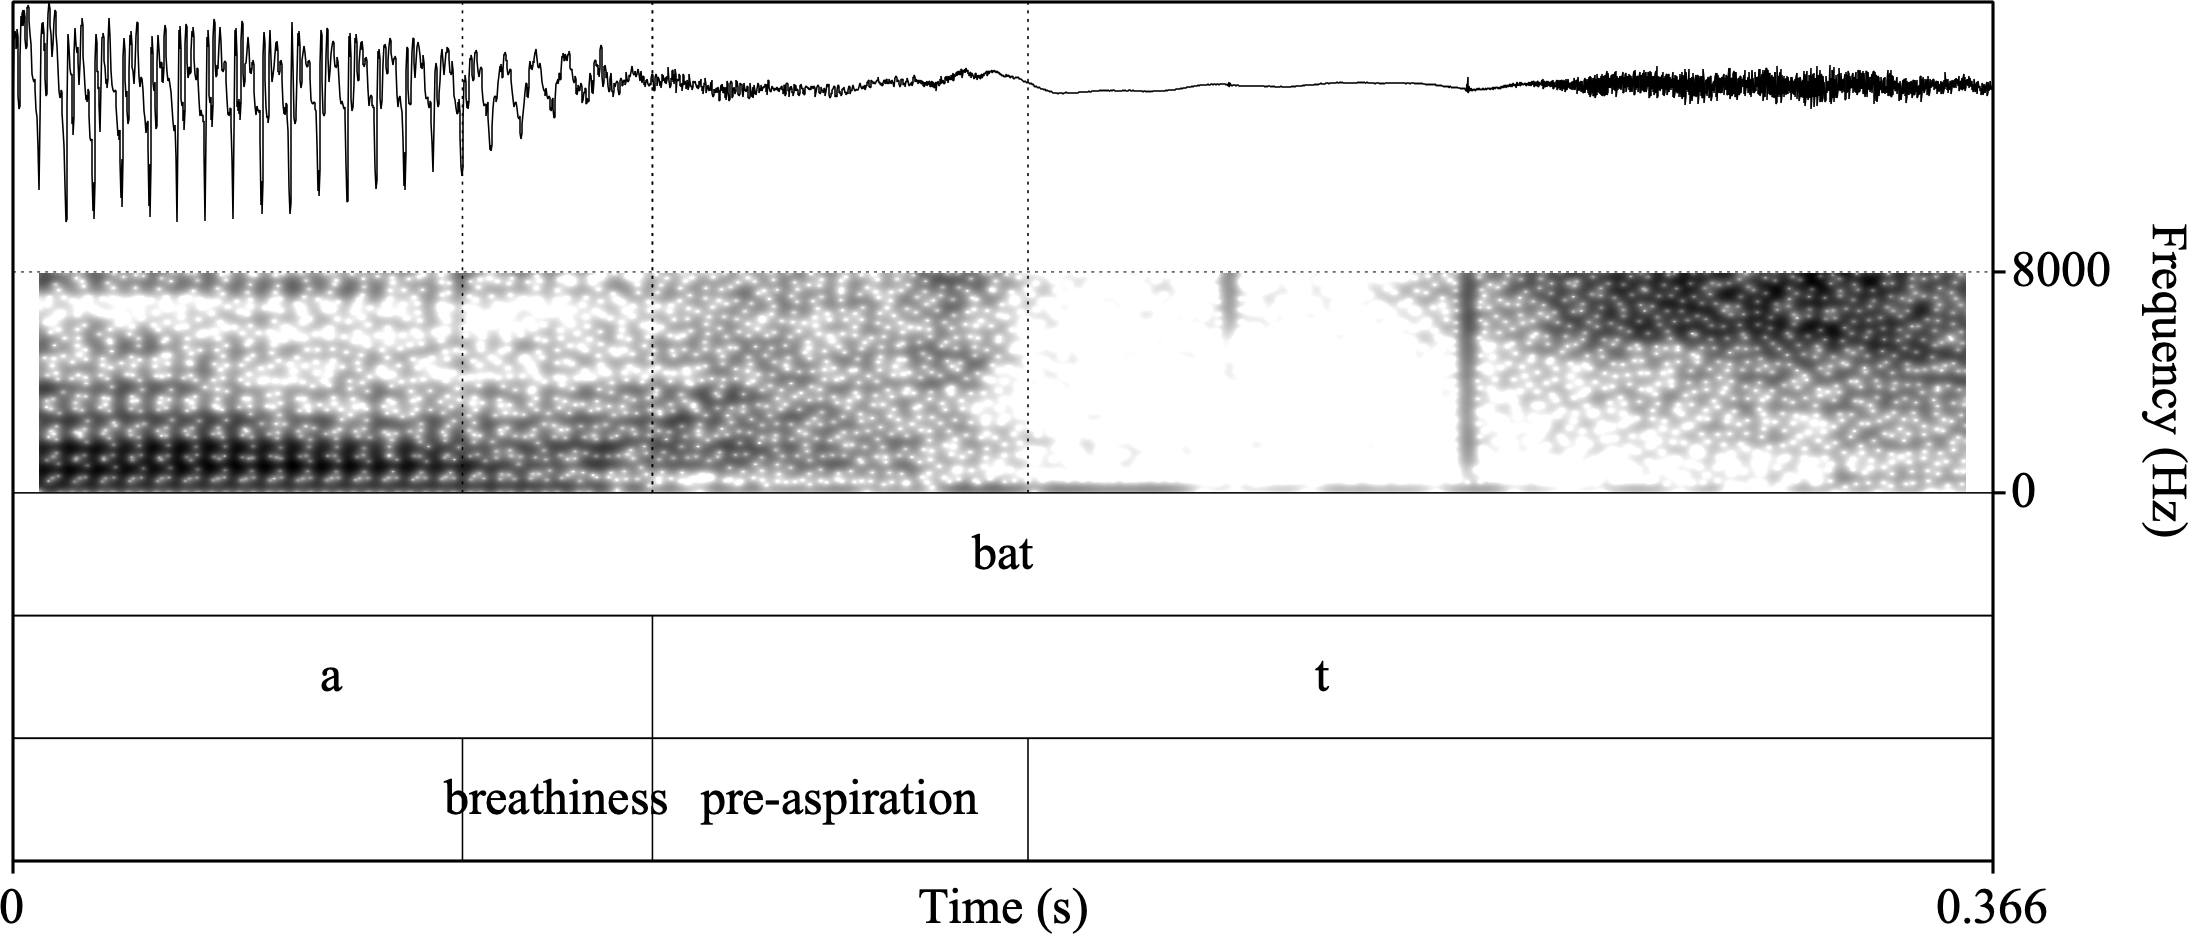
\includegraphics[width=\textwidth]{figures/Hejna-img001.png}
\caption{\label{fig:hejna:1}Example of pre\hyp aspiration in the word \textit{bat}, as produced by a speaker of Welsh English, using acoustic data}
\end{figure}

As is discussed in more detail in \sectref{sec:hejna:2.7}, pre\hyp aspiration frequently manifests itself by a gradual increase of breathiness, which can ultimately lead to the loss of voicing and result in voiceless pre-aspiration. This onset of glottal friction has been measured through Voice Offset Time, or VOffT, by some researchers (e.g. \citealt{Pind1998}), as a measure analogous to Voice Onset Time (VOT) used to analyse the duration of post-aspiration.

Importantly, the literature on pre\hyp aspiration in the languages of the world quickly reveals differences across the definitions of the phenomenon, and formulating an inclusive definition may become a rather cumbersome task as a result. These differences are linked to four factors:

\begin{itemize}
\item[(i)] the nature of the sequences in which pre\hyp aspiration occurs: more specifically, the manner of articulation of both the preceding and the following segments;
\item[(ii)] the presence of voicing: whether only voiceless frication should be considered pre-aspiration;
\item[(iii)] the source of frication in pre-aspiration: whether it is purely glottal, or oral, or both;
\item[(iv)] the status of pre\hyp aspiration as a segment or a sub\slash suprasegment: whether it forms a part of a consonantal cluster hC rather than being part of a single consonantal phoneme.
\end{itemize}

In order to explore the three research questions formulated above, several contentious issues surrounding the phenomenon need to be (re)visited. \sectref{sec:hejna:2} opens with a discussion of what has been seen as pre\hyp aspiration phenomena \citep{Silverman2003}, including “true” or “genuine” pre\hyp aspiration (or pre\hyp aspiration proper), sonorant devoicing, pre-affrication, vowel devoicing, sequences of [h] and consonants, \mbox{/s/} debuccalisation, breathy sonorants, and other related phenomena. As will be shown, different approaches to the definition of pre\hyp aspiration have various consequences for our understanding of the typological behaviour and the frequency of the phenomenon, as also mentioned by \citet[32]{Clayton2010} and \textcitetv{chapters/02_Iosad}. The second contentious issue, introduced in \sectref{sec:hejna:3}, is linked to the phonological status of pre-aspiration. Should typologists consider languages as having pre\hyp aspiration only if pre\hyp aspiration is contrastive? How is contrastiveness established? Is contrastiveness the only diagnostic of the phonological status of a phenomenon? And is it the case that pre\hyp aspiration is rarely contrastive?

Next, the discussion moves to the proposals suggested to explain why pre\hyp aspiration is very rare. The predominant proposal in earlier work is linked to the so-called Perceptual Inferiority Hypothesis (\citealt{Silverman2003, Clayton2010}), according to which pre\hyp aspiration is rare because it is difficult to hear. A review of the extremely limited literature available in this area (\sectref{sec:hejna:4.1}) does not support this hypothesis. However, historical and structural reasons for whether we should expect pre\hyp aspiration to be rare are discussed in \sectref{sec:hejna:4.2}. Finally, practical challenges related, for instance, to the quality of the acoustic signal in the data the researcher may work with are introduced in \sectref{sec:hejna:4.3}.

The conclusion reached in this chapter is that pre\hyp aspiration is rare, but not as rare as suspected, and not necessarily for the reasons put forward in the literature. Most importantly, however, I conclude that very little is known about the phenomenon – possibly too little for us to be able to assess how common pre\hyp aspiration is in the languages of the world. This being the case, the chapter ends with a list of research questions that need to be addressed in future research on pre-aspiration.

Before diving into these issues, however, \sectref{sec:hejna:1.2} provides an overview of languages reported to have pre\hyp aspiration of some type.

\subsection{Which languages have pre-aspiration?}\label{sec:hejna:1.2}
\begin{sloppypar}
With the caveat that different researchers can adopt rather different definitions of the phenomenon, my conclusions are that pre\hyp aspiration has been reported in (at least) 19 languages families and (at least) approximately 84 languages. The 19 language families can be found across the globe, including Afro-Asiatic, Algic, Arawakan, Austronesian, Indo-European, Mongolic-Khitan, Nakh-Dagestanian, Otomanguean, Sino-Tibetan, Siouan, Tarascan, Tucanoan, Tungusic, Turkic, Uralic, Uto-Aztecan, Bora(n)/Witotoan, and Yuchi; and the Urarina isolate. The appendix to this chapter provides a list of these pre-aspirating languages by language family (Tables 1--19). Needless to say, estimating the exact number of languages reported to have pre\hyp aspiration is rendered challenging by the fact that distinguishing languages and dialects is not straightforward. Furthermore, the definition of pre\hyp aspiration provided in the previous section generally covers pre\hyp aspiration which might be considered prototypical. This prototypical pre\hyp aspiration has been referred to with the following terms: genuine pre\hyp aspiration \citep{Silverman2003}, prototypical pre\hyp aspiration \citep[86]{Clayton2010}, pre\hyp aspiration proper (e.g. \citealt{Helgason2002,Helgason2003}), and true pre\hyp aspiration (e.g. \cites[132]{TorresKasak2019}[24]{Helgason2002}[25]{KoremanEtAl2008}). However, the term “pre-aspiration” has also been used for other phonetic and phonological phenomena, as will be shown in the next section. This necessarily impacts the estimated number of pre-aspirating languages.
\end{sloppypar}

\section{The pre\hyp aspiration collective}\label{sec:hejna:2}

A definition of a linguistic phenomenon necessarily affects our estimates regarding how frequently it is found in the languages of the world. As \citet[576]{Silverman2003} states, “[w]hile primary sources sometimes acknowledge that “pre-aspiration” is indeed a cover term for a variety of phonetic configurations, the secondary literature is typically remiss in carefully documenting this variability”. A range of phenomena have been referred to as pre\hyp aspiration by different researchers:

\begin{itemize}
\sloppy
\item pre\hyp aspiration (also “true” or “genuine” pre-aspiration, pre\hyp aspiration “proper”);
\item pre-affrication (or pre-spirantisation);
\item sonorant devoicing;
\item /s/ debuccalisation;
\item /hC/ clusters;
\item vowel devoicing (or vowel aspiration);
\item glottalisation\slash laryngealisation.
\end{itemize}

To what extent does this menagerie of pre\hyp aspiration consist of phenomena that may perhaps not be cases of pre-aspiration? Each phenomenon is considered briefly in the remainder of this section, focusing on why these may and have been considered pre\hyp aspiration by some but not by others. For reasons of space, the aim is to focus on the overall overview rather than go into language-specific (and often complex) debates.

\subsection{Pre-affrication and pre-spirantisation}\label{sec:hejna:2.1}

\citegen[529]{Silverman2003} overview of pre-aspirating languages brings our attention to the fact that most pre-aspirating languages do not necessarily involve glottal friction in the phonetic implementation of pre-aspiration. Instead, they employ oral friction, or what Silverman refers to as pre-spirantisation. Thus, Chamicuro (Arawakan) is reported to have glottal friction while Goajiro (Arawakan) is reported to have oral friction as the phonetic realisation of pre-aspiration. 

Indeed, Silverman points out that this oral realisation of the phenomenon seems to be so common that pre\hyp aspiration realised as \textit{glottal} friction is actually even rarer (\citeyear[575]{Silverman2003}). To reason why pre\hyp aspiration is cross-linguistically realised with oral and not (just) glottal friction has been linked to perception. \citet[575]{Silverman2003} notes that glottally realised pre\hyp aspiration can develop into orally realised “pre-aspiration” in order to become perceptually more salient (see also \cites[111--112]{Blevins2004}[1, 4, 57--58, 213]{Kehrein2002}). It is challenging to assess just how frequent oral variants of pre\hyp aspiration are cross-linguistically; however, \citet[117]{Clayton2010} proposes that this is “probably quite a widespread phenomenon”. There is also an articulatory link between the two. \citet[124]{EslingEtAl2019} point out that the amount of airflow passing through the larynx in the production of pre\hyp aspiration can be manipulated in order to increase the turbulence and the perceived noisiness of the phenomenon. Thus, there is variation in the noisiness levels of pre\hyp aspiration not only when contrasting oral and glottal realisations, but also at the level of the larynx as a whole, and no doubt within oral realisations as well.

Variation is found not only across languages and speakers but within individual speakers as well. I would like to show an example from my own (Welsh English) data, in which friction with rather different spectral profiles can be found. Examples like those shown in Figures 2 and 3 are very common in my corpus.

  
\begin{figure}
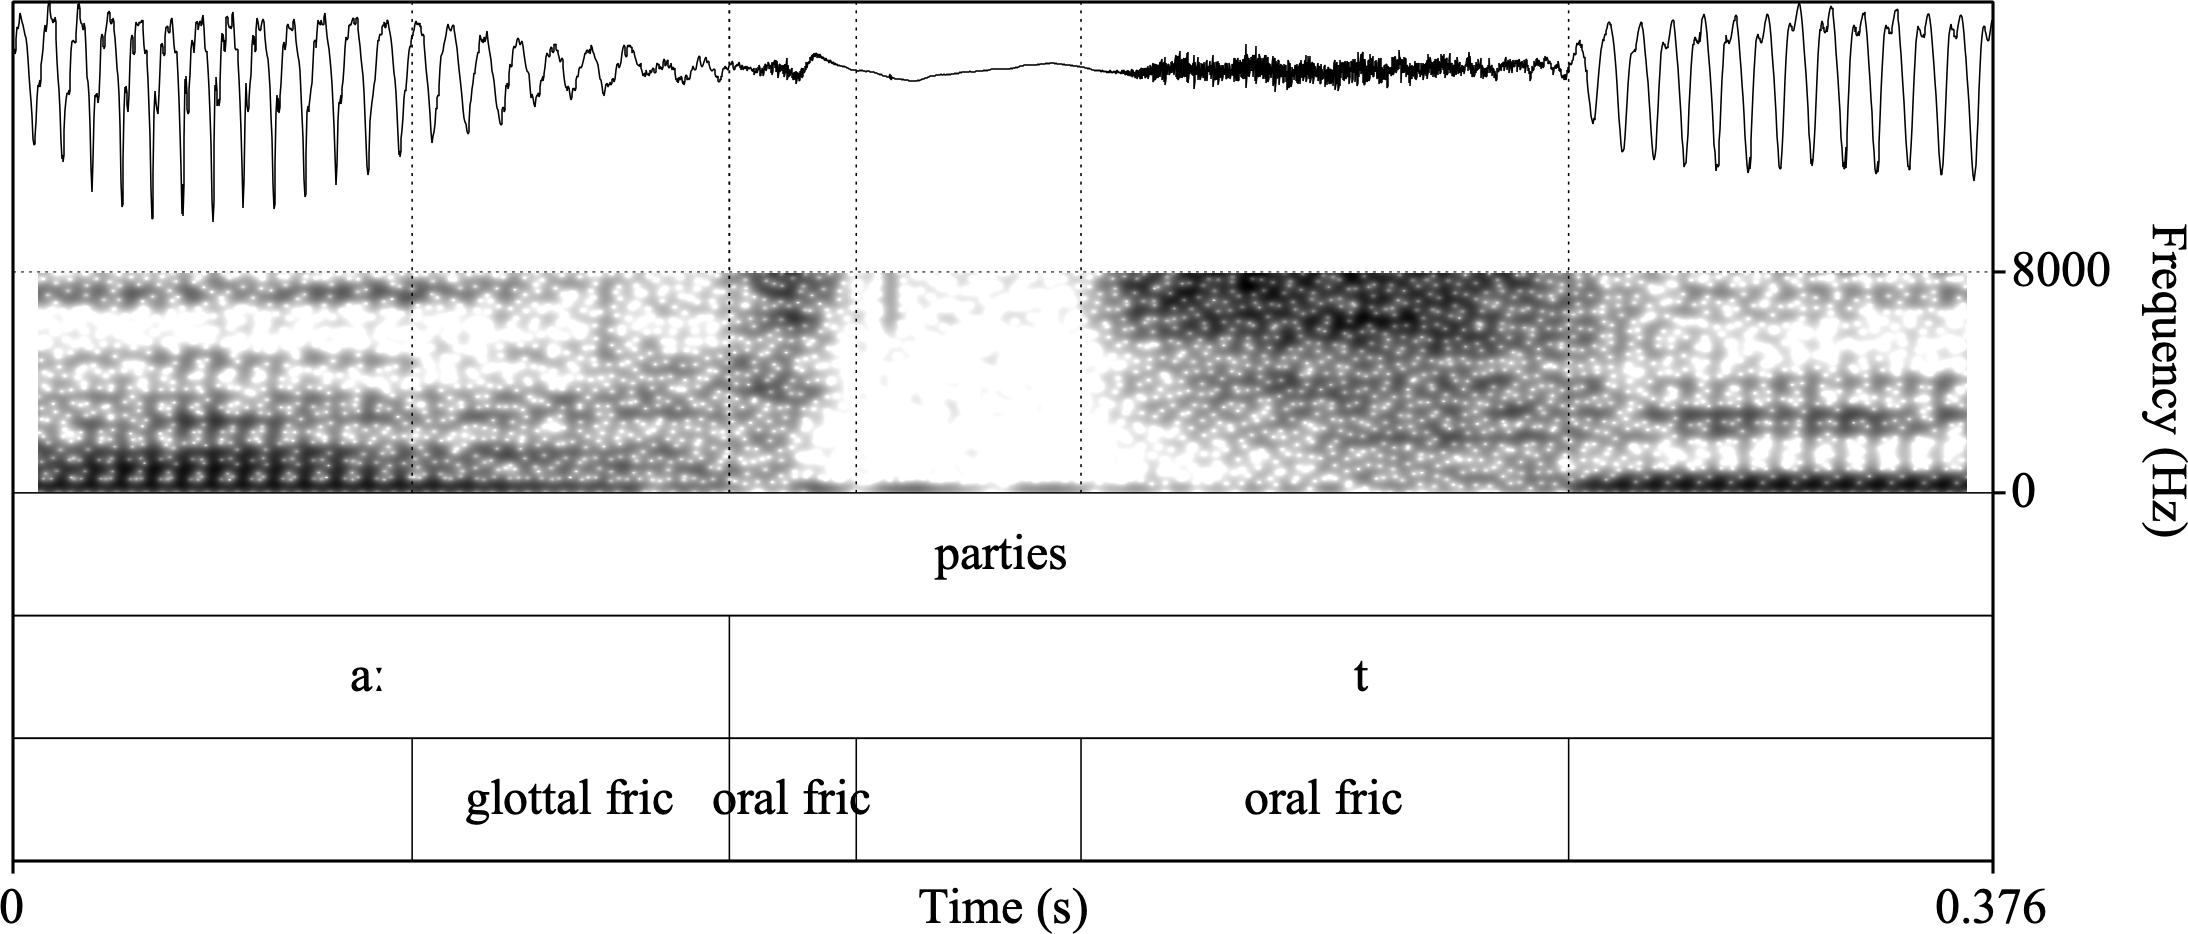
\includegraphics[width=\textwidth]{figures/Hejna-img002.png}
\caption{\label{fig:hejna:2}Example of pre\hyp aspiration in the word \textit{parties}, as produced by a speaker of Welsh English, using acoustic data. Abbreviations: ``glottal fric'' = glottal friction; ``oral fric'' = oral friction}
\end{figure}

  
\begin{figure}
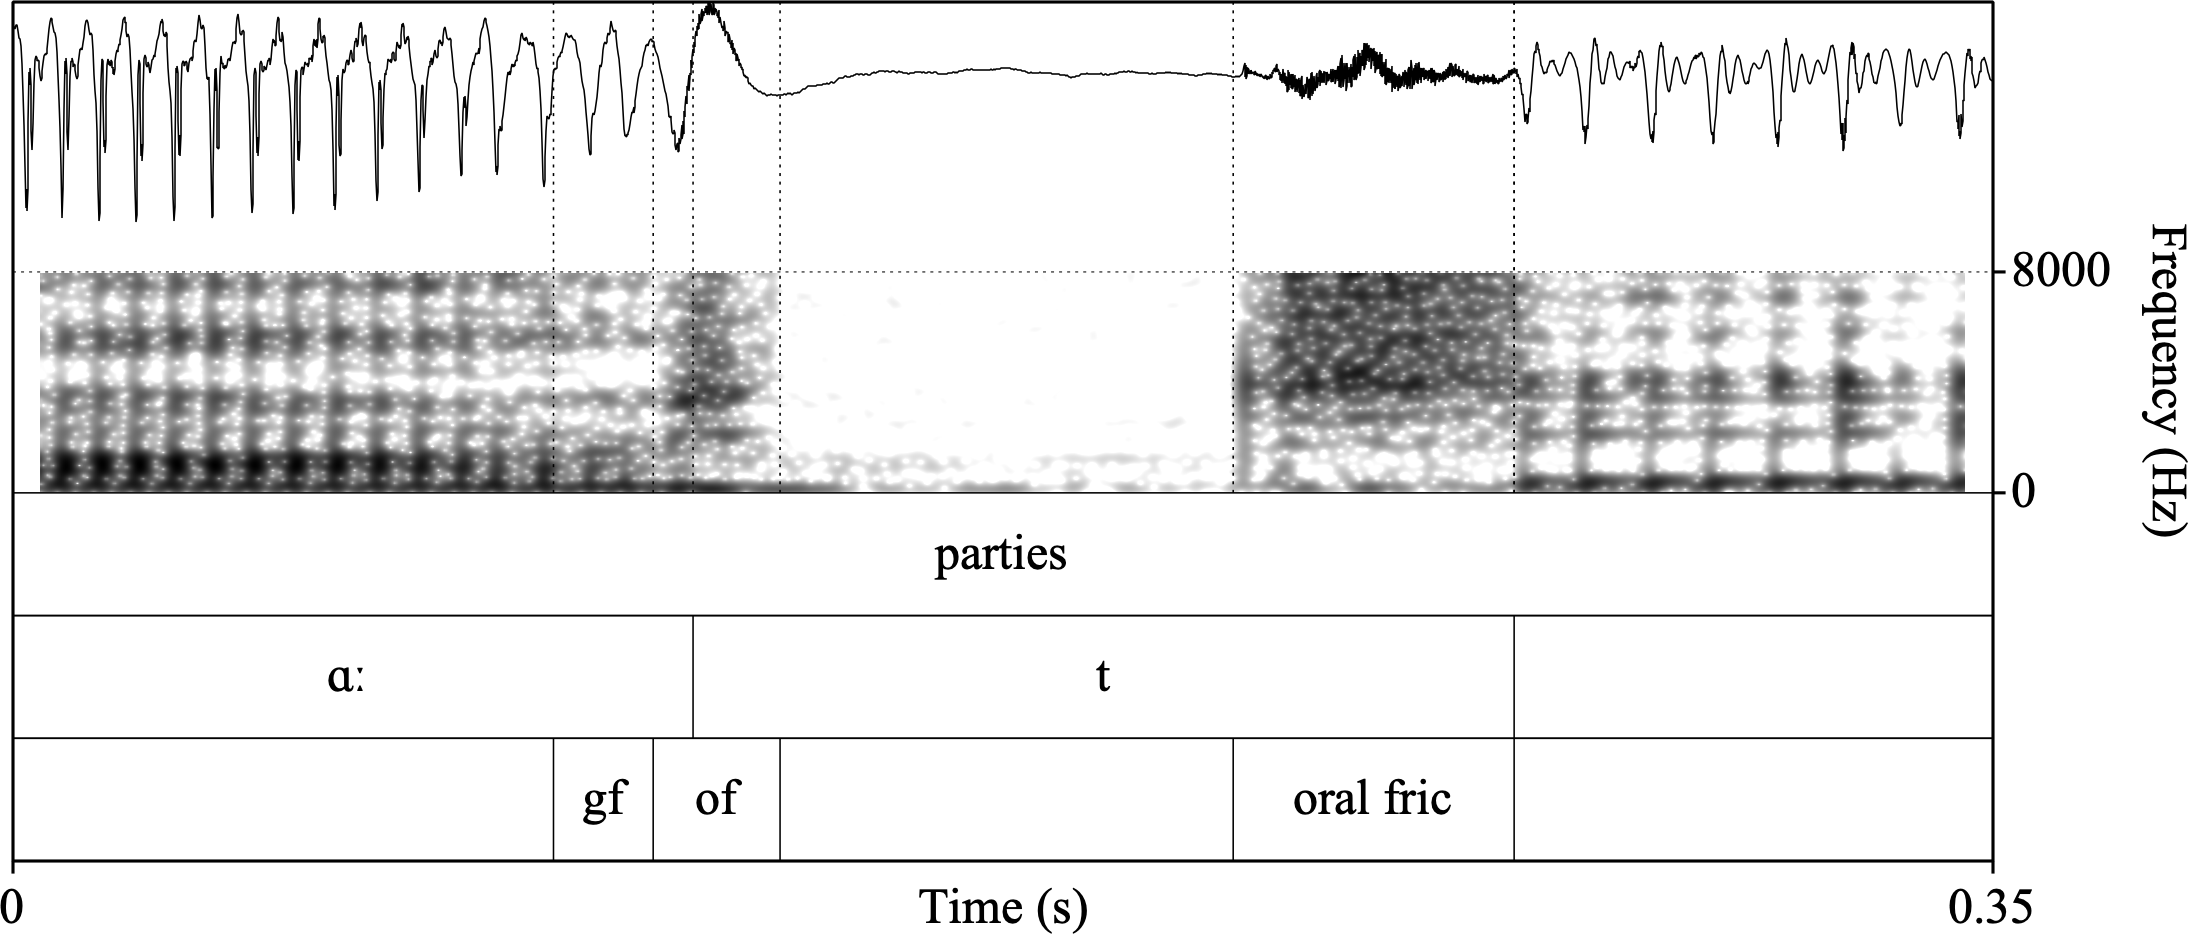
\includegraphics[width=\textwidth]{figures/Hejna-img003.png}
\caption{\label{fig:hejna:3}Example of pre\hyp aspiration in the word \textit{parties}, as produced by a speaker of Welsh English, using acoustic data. Abbreviations: ``gf'' = glottal friction; ``of'' and ``oral fric'' = oral friction}
\end{figure}

The annotations in Figures 2--3 show acoustic events that could be labelled “glottal friction” and “oral friction”, to employ the two categories highlighted by \citet{Silverman2003}. While glottal friction usually displays a fairly even distribution of lower-intensity energies across a range of frequencies, oral friction tends to be concentrated at specific frequencies which depend on the quality of the sound in question (e.g. \citealt{Fry1982}). In the absence of articulatory data, which most phoneticians working on pre\hyp aspiration do not have at their disposal, instances such as those found in Figures 2--3 might be labelled as partially pre-spirantised or pre-affricated (for pre-affrication, see \citealt{Laver1994}: 150--151). However, we need to bear in mind that higher-intensity energy in and of itself does not necessarily signal an oral source, and spectral properties should be carefully examined. One fact is nevertheless undoubtedly certain: pre\hyp aspiration is realised with a range of phonetic variants, and a single token can display sequences of variably turbulent friction.

Pre-aspiration realised with primarily oral friction should be included in typological overviews of the phenomenon. Indeed, spectral properties of pre\hyp aspiration (and those of post-aspiration) are a very important aspect to consider: \citet{Silverman2003} argues that pre\hyp aspiration is not a mirror image of post-aspiration because the latter lacks orally generated friction. However, work by \citet{Hejná2015, Hejná2016b} and \citet{NanceStuart-Smith2013} suggests that post-aspiration is spectrally more varied as well. We should therefore adopt more varied approaches towards acoustic analyses of post-aspiration and pre\hyp aspiration which would go beyond our use of Voice Onset Time\footnote{Maddieson (p.c. 2021) expressed similar sentiments to me with respect to (post-)aspiration in Thai and Navajo.} and Voice Offset Time, respectively, as the sole or predominant analytical tools.

\subsection{Sonorant devoicing}\label{sec:hejna:2.2}

Another phenomenon very closely linked to aspiration in general is sonorant devoicing, as in, for instance, pre-plosive sonorant devoicing in Welsh English \textit{milky} [mɪl̥kʰɪ]; and post-plosive sonorant devoicing in \textit{train} [tɹ̥eɪn]). The term “sonorant devoicing” refers to the devoicing of consonantal sonorants. Several pre-aspirating languages have been noted to show sonorant devoicing as well (e.g. Faroese, Icelandic, Lule Sámi, Swedish, cf. \cites[70]{LadefogedMaddieson1996}[11]{Helgason2002}). Various researchers have treated sonorant devoicing as a manifestation of pre\hyp aspiration (e.g. \citealt[70]{LadefogedMaddieson1996}, and other researchers mentioned in \citealt{Helgason2002}: Section 2.2 in particular).

There is a good reason why pre\hyp aspiration and sonorant devoicing should be considered together: they seem to be closely linked both from a synchronic and a diachronic point of view. Indeed, \citet[70]{LadefogedMaddieson1996} discuss pre\hyp aspiration in both VC (vowel-consonant) and NC (sonorant-consonant) sequences under the phenomenon of pre-aspiration. \citet{Hejná2016c} proposes that pre\hyp aspiration first innovates in the sequences of vowels and phonetically voiceless obstruents and then spreads to environments which include sonorant consonants as well. In this view, pre\hyp aspiration and sonorant devoicing could be seen as phonotactically determined realisations of the same phenomenon.

Despite the fact that sonorant devoicing preceding voiceless obstruents has been considered part of a more general process of pre-aspiration, the terms “pre-aspiration” and “sonorant devoicing” or “sonorant voicelessness” have nevertheless been used for the two segmentally different contexts (pre-aspiration for vowels, sonorant devoicing for sonorant consonants). Researchers studying pre\hyp aspiration thus need to be wary that the term “pre-aspiration” is primarily used in the literature for sequences including first of all vowels (but sometimes also sonorant consonants) and “sonorant devoicing” for sequences including sonorant consonants.

\subsection{The question(s) of /hC/ clusters and debuccalisation of /s/}\label{sec:hejna:2.3}
\subsubsection{Pre-aspirated singletons vs /hC/ clusters}

One of the thorniest aspects surrounding the typology of pre\hyp aspiration pertains to the decisions whether a language does indeed have pre-aspirated consonants or clusters of \mbox{/hC/} instead. More generally, \citet[9, 33]{Clayton2010} treats instances of [h] before voiceless non-continuants (including plosives and affricates) as pre-aspiration, while cases with [h] which can occur in other consonantal contexts as forming a cluster. For \citet[33]{Clayton2010}, pre\hyp aspiration is therefore a feature restricted to plosives and affricates. However, if a language shows [h] not only in the vicinity of voiceless plosives but also near other consonants, [h] in the vicinity of a voiceless plosive is not considered by him to be a case of a pre-aspirated plosive but rather a case of an \mbox{/hC/} cluster. Clayton, therefore, does not include languages such as Chamicuro (Arawakan), Finnish (Uralic), Huatla Mazatec (Otomanguean), and Spanish (Indo-European) in the list of pre-aspirating languages, while some other researchers do (see Tables 1--19). \citet{KehreinGolston2004} present a somewhat more radical approach to the issue at hand, namely, the Prosodic Account. In this framework, laryngeal specifications are delegated to the realm of prosody rather than (directly) that of segments. This has implications for the debates connected to languages where it is not clear whether pre\hyp aspiration is part of a segment or indeed a consonantal segment in a cluster. More specifically, \citet{KehreinGolston2004} and \textcite[90, 98, 100, 117, 213]{Kehrein2002} predict that these two options (/pʰ/ vs /ph/) are never contrastive, which seems to be borne out by the data found in the languages of the world (also \cites[79]{Steriade1992}{Steriade1994}).

Such debates clearly have implications for which languages “make it” to the list of pre-aspirating languages. To provide some contested examples, \citet[132]{TorresKasak2019} discuss Hidatsa (Siouan) and its “<hC> elements”, and conclude that these do not present pre-aspiration.\footnote{I have not been able to identify clear reasons for this in their paper. This is because it seems to be assumed right from the beginning that “<h>” is a segment (and, therefore, not pre-aspiration).} In addition, \citet[25]{Helgason2002} mentions Comanche and Mono (Uto-Aztecan) as languages for which the pre\hyp aspiration vs cluster debates are ongoing. The arguments put forward in individual studies are diverse and can require an in-depth understanding of the phonological system of the language in question, including its historical development. \Citeauthor{chapters/18_vantveer} (\citeyear{chapters/18_vantveer}) present an apt example. The authors analyse pre-consonantal [h] in Ecuadorian Siona (Tukanoan) in order to shed light on whether the language has pre\hyp aspiration or a /hC/ cluster. They conclude that the phenomenon is pre-aspiration, despite the synchronic co-occurrence of [h] not only with obstruents but also with /ɲ/. This is because the pre-nasal [h] is analysed as having a phonemic status and not as part of the pre\hyp aspiration process operating in the language. This situation is accounted for through both diachronic and synchronic analyses.

\subsubsection{Debuccalisation of /s/}
\largerpage
Debuccalisation of /s/ plays an important role in typological discussions of pre-aspiration. As we will see, it is also very much linked to the debates on pre-aspirated singletons vs /hC/ clusters.

Debuccalisation includes a range of processes whereby an orally articulated segment becomes articulated primarily by the laryngeal articulator \citep{EslingEtAl2019}. Debuccalisation examples include such processes as [s] → [h] or, for instance, [t] → [ʔ]. Pulmonic sounds are not the only ones that can undergo debuccalisation \citep{Fallon1998}. As \citet[200]{Fallon1998} notes, debuccalisation is “a common process which recurs in many language families all over the world”. Debuccalisation of /s/ in the environment of voiceless plosives (e.g. [sk] → [hk] {\textasciitilde} [ʰk]) is a contentious issue in the pre\hyp aspiration literature. On the one hand, we find approaches such as those by \citet[593]{Silverman2003}, who very explicitly mentions “[s]-stop clusters” as a common historical source of pre-aspirated plosives. On the other hand, some approaches explicitly reject languages with debuccalisation as pre-aspirating. This is because such cases may be considered consonantal clusters rather than pre-aspirated singletons.

The discussion of [s]-stop clusters giving rise to [h]C (i.e., pre-aspirated consonants, at least on the surface) nevertheless does frequently refer to the process of debuccalisation as a historical source of pre-aspiration. This includes much of the work on pre\hyp aspiration in dialects of Spanish (e.g. see \citealt{Chappell2014,Chappell2015, CronenbergEtAl2020, Torreira2007}, and the references therein). Interestingly, pre\hyp aspiration in Icelandic – one of the most well-known pre-aspirating languages – has also been interpreted by some as originating in the process of debuccalisation, albeit one which involves geminates \citep[36]{Fallon1998}. Although these geminates nevertheless consist of geminated plosives, this example shows that debuccalisation cannot be avoided in typological discussions of pre-aspiration.

The take-home message of this section is that, for many languages, debates linked to the status of [h] as pre\hyp aspiration are ongoing, and it is not clear what (synchronic and/or diachronic) criteria should be used to reach an answer that would leave everyone satisfied. 

\subsection{Vowel devoicing}\label{sec:hejna:2.4}
\largerpage
\dictum[(\citealt{Windsor2016}: 67)]{“The question now is how do consonantal aspiration and vowel devoicing relate to one another, if they do at all.”}
\vskip\baselineskip
\noindent
Vowel devoicing, or vowel aspiration, is another phenomenon which is sometimes referred to as pre-aspiration.\footnote{See also \citet[204]{Jensen2000} for a discussion of post-aspiration as a voiceless vowel.} Some researchers have in fact defined pre\hyp aspiration as involving vowel devoicing (e.g. \citealt{KarlssonSvantesson2011}: 121). In such cases, the two terms seem to be used either interchangeably or in a way such that pre\hyp aspiration presents a specific type of vowel devoicing. Others nevertheless distinguish between the two (e.g. \cites{Stenzel2004,MillerEtAl2005,Elias-UlloaAramburú2021}[90--117]{Liberman1982}). The former approach is substantiated by the fact that most of the studies focusing on pre\hyp aspiration report the phenomenon in the sequences of vowels and phonetically voiceless obstruents. A considerable amount of ink has been spilt over the questions surrounding the affiliation of pre-aspiration, i.e. whether pre\hyp aspiration should be considered part of the consonant, of the vowel, of both, or of neither (e.g. \citealt{Hejná2015}: 33--36, 65--66). Pre-aspiration does present us with a certain unavoidable indeterminacy, considering its traditional presence in the sequences of sonorants (vowels and sonorant consonants) and obstruents. The presence of pre\hyp aspiration in exactly this segmental environment results in its phonetic realisation as typically reflecting a change from the voicing of a vowel or a sonorant consonant to the voicelessness of an obstruent. Looking back to \figref{fig:hejna:1} above, we can see that the voiceless glottal friction labelled “pre-aspiration” (voiceless pre-aspiration) is preceded by local breathiness (voiced component of pre-aspiration). The role of local breathiness is discussed further below in \sectref{sec:hejna:2.7}. The local breathiness is important as it shows that in the sequences of vowels and phonetically voiceless obstruents, we typically see a transition from a more modal to a less modal vowel. The transition is caused by laryngeal abduction, which increases and ends up in voicelessness – voiceless aspiration, or indeed what most researchers would consider to be pre-aspiration.

However, “vowel devoicing” is a term familiar primarily from the literature focusing on languages such as Japanese and French (e.g. \citealt{Tsuchida2001, Smith2003}). There are two important similarities between what is normatively referred to as “pre-aspiration” and “vowel devoicing”. Firstly, laryngeal abduction occurs in the context of a vowel. Secondly, the process of abduction, which can lead to partial and full devoicing (i.e. including voiceless friction), is conditioned primarily by voiceless segments.

There are nevertheless also some differences between “pre-aspiration” and “vowel devoicing”. Firstly, pre\hyp aspiration is more frequent and longer in duration with low vowels (cf. \cites[107--108]{Hejná2015}[17]{MorrisHejná2020}, for overviews), while vowel devoicing is rather favoured by high vowels \citep[65]{Ohala2011}. Secondly, pre\hyp aspiration is not reported to emerge in the sequences of a pause plus a vowel (e.g. pause + \textit{aloe}) and a vowel plus a pause (e.g. \textit{Ha!} + pause, \textit{uh} + pause), while vowel devoicing is (e.g. \cites[193]{Smith2003}{Tsuchida2001}). Indeed, the two main historical sources of vowel devoicing identified in the literature include, firstly, a typically short vowel surrounded by voiceless segments and, secondly, an occurrence of a vowel at a domain edge (e.g. \cites[199]{Blevins2004}{Kuznetsova2015}). Thirdly, although pre\hyp aspiration has been reported to result in full devoicing of a vowel (\citealt{JatteauHejná2016}: 16), in my own experience with data from English dialects, Halh Mongolian, and Welsh, this seems to be extremely rare, occurring in two out of approximately 9,000 tokens. Those are the contexts where the vowel is surrounded by heavily aspirated obstruents. On the other hand, vowel devoicing is frequently reported to affect the entire vowel segment (\cites[1--2]{OberlyKharlamov2015}{KuznetsovaVerkhodanova2019}). Fourthly, pre\hyp aspiration is preferred in stressed environments (e.g. \citealt{HejnáJespersen2019}: 241--242, see also \citetv{chapters/18_vantveer} and \citetv{chapters/17_Craioveanu}), whereas vowel devoicing seems to be favoured in unstressed environments (see e.g. the discussion in \citealt{Smith2003}). 

These observations are not based on a comprehensive inspection of the literature. Instead, they are primarily meant to initiate a discussion for future research in order to tease apart instances of vowel devoicing and pre\hyp aspiration (or indeed also different types of what could be considered vowel devoicing). However preliminary the observations above may be, they nevertheless indicate that pre\hyp aspiration and vowel devoicing are rather two different phenomena. They may also be phonetically fairly similar but functionally different, and so the decision in each case would require an in-depth analysis of segmental and prosodic conditioning, and of whether a vowel is found to be fully devoiced or not (and how frequently). Unfortunately, not all sources that discuss pre\hyp aspiration provide a sufficient amount of detail for this (see also \citealt{Silverman2003}: 577).

This being the case, unless more research is conducted, we may not always be able to conclude whether we are dealing with vowel devoicing or pre\hyp aspiration for the languages in the descriptions of which both terms have been used. A case in point is Udihe (Tungusic). According to \citet[126, 300]{Liberman1982}, Udihe – or what he refers to as Ude(ge) – is a language in which pre\hyp aspiration can be found. However, this information is conveyed in form of a passing comment, and it is unclear where this information actually comes from. An in-depth analysis reveals that Udihe exhibits vowel devoicing (partial or full aspiration) rather than any kind of normatively defined consonantal pre\hyp aspiration \citep{Kuznetsova2022}. \citet{OberlyKharlamov2015} provide another relevant case with their analysis of Southern Ute (Uto-Aztecan). Discussions surrounding pre-aspiration/vowel devoicing in Blackfoot (Algic) also present a very relevant example (\citealt{ReisSilva2008}). Similarly, \textcitetv{chapters/18_vantveer} touch upon pre\hyp aspiration being discussed as vowel devoicing in Siona and Western Tukanoan languages. The need for more in-depth work in this area is also voiced by \citet[55]{Stenzel2004}.

\subsection{Glottalisation/laryngealisation}\label{sec:hejna:2.5}

Finally, to a limited extent, we find that some researchers use the terms “laryngealisation” and/or “glottalisation”, and/or “pharyngealisation” to (potentially) discuss pre-aspiration. \citet[149]{Hejná2015} provides an example of a relevant discussion which may be challenging to make sense of by the readers. In his discussion of “pseudo-støds and related phenomena” in Tuvan (Turkic), Ket (Yeniseian), and Ude(ge) (Tungusic), \citet[126--127]{Liberman1982} equates the term “pre-aspiration” with “pharyngealisation” and what might also be glottalisation.\footnote{\citet{Kuznetsova2022} mentions that the phenomenon in question in Tuvan and in a related language Tofa is usually referred to as “vowel pharygealisation”, while her field data (Kuznetsova, p.c., 2022) rather shows vowel laryngealisation/glottalisation. Furthermore, I am informed that glottalisation shows no traces of breathiness there, and this is the case in Ket as well (see references in \citealt{Kuznetsova2022}).}

It may be challenging to discern from these descriptions whether the phenomenon in question is laryngeal friction produced by glottal abduction or not. For instance, \citet[427]{Dwyer2000} refers to a “glottalised \textit{h} stem” in some Turkic languages in a discussion of subsegmental pre\hyp aspiration and pre\hyp glottalisation. However, she provides transcriptions showing pre\hyp aspiration, which may be somewhat confusing for the reader. In other work, we also find cases in which glottalisation or laryngealisation is mentioned – very explicitly and unambiguously – as a possible realisation of pre-aspiration. For example, \citet[4]{KarlssonSvantesson2012} report that “[p]re-aspiration often manifests itself as laryngealisation of the preceding vowel” in their data from selected Mongolic, Turkic, and Tungusic languages. Similarly, \citet{StevensHajek2007} mention pre-glottalisation as one of the possible realisations of pre\hyp aspiration in their Sienese Italian data.

The reason why some confusion can be found in sources might be explained by the fact that pre\hyp aspiration and pre\hyp glottalisation can co-occur within the same token. Indeed, laryngeal abduction and laryngeal adduction are not necessarily mutually exclusive (\citealt{Hejná2023, MoisikEtAl2022}), although they have been known to be contrastive in some languages, such as Udihe \citep{Kuznetsova2022}, and are represented with the two different laryngeal features [spread glottis] and [constricted glottis] in various phonological frameworks. \citet{Hejná2023} shows examples of simultaneous production of pre\hyp aspiration and pre\hyp glottalisation in Welsh English, which she interprets as local whispery and/or breathy creak. \citet{KarlssonSvantesson2011} further discuss intriguing examples of pre\hyp aspiration inducing creakiness in present-day Mongolian dialects. \textcitetv{chapters/12_WatsonEtAl} in turn draw attention to the production of sonorants by a Mehri (Afro-Asiatic) speaker whose acoustic evidence shows the presence of glottalisation, while the electroglottographic evidence suggests the presence of glottal abduction. For a brief general discussion (with a focus on English data) of the relationship between pre\hyp aspiration and (pre-)glottalisation in voiceless obstruent contexts from a diachronic and a synchronic perspective, see \citet[Ch. 5]{Hejná2015}.

To provide an interim summary, all the phenomena discussed in this section (Sections \ref{sec:hejna:2.1}-\ref{sec:hejna:2.5}) can be and have been treated as different from pre\hyp aspiration and from one another. Nevertheless, they can very often be connected via a range of synchronic and diachronic links, depending on the language in question. As we have also seen, we do not always (as yet) have sufficiently in-depth data available in order to resolve questions of this type. In the remainder of this section (Sections \ref{sec:hejna:2.6}-\ref{sec:hejna:2.7}), two final issues which are relevant to fundamental definitional aspects of pre\hyp aspiration are discussed. Firstly, pre\hyp aspiration is not found solely in the context of plosives (or stops), as discussed in \sectref{sec:hejna:2.6}. Secondly, different approaches to how pre\hyp aspiration is quantified follow from how the phenomenon is defined, even in cases where the definition would fall within what has been labelled as “true pre-aspiration” above (\sectref{sec:hejna:2.7}).

\subsection{It’s not just plosives}\label{sec:hejna:2.6}
\subsubsection{Pre-aspirated obstruents}\label{sec:hejna:2.6.1}

Two of the major works on the typology of pre\hyp aspiration target pre-aspirated plosives rather than pre-aspirated obstruents (\citealt{Silverman2003, Clayton2010}). At least three other PhD theses have been dedicated to pre-aspiration, and these too show a strong focus on pre-aspirated oral plosives. \citegen{Chasaide1985} work specifically analyses Icelandic, Irish, and Scottish Gaelic through a range of in-depth acoustic, articulatory, and perceptual analyses of plosives. \citet{Helgason2002} discusses the history of pre\hyp aspiration in Scandinavian languages. Helgason primarily relies on acoustic and perceptual analyses of pre-aspirated plosives, but includes a discussion of pre-aspirated fricatives as well. \citet{Hejná2015} offers detailed acoustic analyses of Aberystwyth English (i.e., Welsh English) pre-aspiration. This work, too, is primarily concerned with plosives, with pre-aspirated fricatives discussed noticeably less so. Does the inclusion of fricatives (and affricates) change our understanding of how frequent pre\hyp aspiration might be in the languages of the world?

To the best of my knowledge, pre-aspirated fricatives have been reported in English (Indo-European; \citealt{HejnáEtAl2021}), Swedish (Indo-European; \citealt{Helgason2002}: 89), Western Yugur (Turkic; \citealt{Roos1998}: 30), and – depending on the analysis~– also in Blackfoot (Algonquian; \citealt{Windsor2016}: 75), Chamicuro (Arawakan; \citealt{Silverman2003}\footnote{\citet[61]{Clayton2010} rejects the analysis of the phenomenon as pre\hyp aspiration in Chamicuro, as also mentioned in \sectref{sec:hejna:2.3} and \sectref{sec:hejna:2.6.2}.}), Forest Nenets (Uralic; \citealt{Salminen2007}), Kickapoo and Menominee (Algic; \citealt{Gathercole1983}), Salar and Kälpin Uyghur (Turkic; \citealt{Dwyer2000}: 427), and Shetland Norn (Indo-European; \citealt{Knooihuizen2013}). \citet[89]{Helgason2002} actually concludes that “preaspiration is not a particular feature of stops, but a general characteristic in production of voiceless consonants”, which is also supported by \citet[9]{Clayton2010}.

Importantly, however, all of these languages have pre-aspirated plosives as well. It therefore seems that the presence of pre-aspirated fricatives implies the presence of pre-aspirated plosives, but the presence of pre-aspirated plosives does not imply the presence of pre-aspirated fricatives. This corresponds to what we observe for post-aspiration, which is more common with plosives than with fricatives (e.g. \citealt{Jacques2011}, and the references therein). Scottish Gaelic (Indo{}-European) has been explicitly commented on as lacking pre\hyp aspiration in fricatives (e.g. \citealt{Clayton2010}: 17), as has Urarina (isolate; \citealt{Elias-UlloaAramburú2021}: 140). Halh Mongolian is another example of a language which has pre-aspirated plosives but not fricatives (\citealt{JatteauHejná2018}).

The absence of pre\hyp aspiration in fricatives is, however, not necessarily commented on explicitly in work on pre-aspirating languages. This challenge has been more generally noted by \citet[577]{Silverman2003}, and also by \citet[17]{Clayton2010}: “Holmer [1949] provides no indication that voiceless fricatives are also preaspirated in Goajiro, which would be telling, but neither does he rule it out”. Generally, it is challenging to know whether absence of an explicit comment on pre\hyp aspiration in the fricative context means that pre\hyp aspiration is not found in this context in the language in question, or if the authors did not look for it.

Scottish Standard English (\citealt{GordeevaScobbie2013}) might present an apparent contradiction to the general observation that a language with pre-aspirated fricatives also has pre-aspirated plosives. \citet[262]{GordeevaScobbie2013} report pre-aspirated fricatives but not pre-aspirated plosives in their data: the plosives are reported to be pre-glottalised.\footnote{For a brief discussion of glottalisation blocking pre-aspiration, see \citet[204]{HejnáKimper2019}, \citet{Hejná2021}, and \citet[216--217]{HejnáEtAl2021}}. The same pattern (VʰF but VˀP, as in \textit{mass} [maʰs] and \textit{mat} [maˀt]) has been found also elsewhere (cf. \citealt{HejnáScanlon2015} on Manchester English). However, it seems to be limited to word-final obstruents (e.g. \textit{mush}, \textit{mutt}) rather than, for instance, word-medial obstruents (e.g. \textit{mushy}, \textit{mutter}). In the latter, pre\hyp aspiration can be found. Word-medial tokens were not included in the Scottish Standard English analysis by \citet{GordeevaScobbie2013}, and we therefore cannot conclude whether Scottish Standard English might be a counterexample to what seems to be a robust tendency.

Having analysed 18 Aberystwyth English speakers with varying degrees of pre\hyp aspiration and pre-glottalisation in their fortis obstruent production, \citet[183]{Hejná2015} suggests that pre\hyp aspiration might develop in post-aspirated plosives first, and spread to fricatives only afterwards. If this proposal is on the right track, the presence of pre\hyp aspiration in fricatives should not affect our current general picture (predominantly based on the distribution of pre-aspirated plosives) of how frequent pre\hyp aspiration is in the languages of the world.

\subsubsection{Pre-aspirated sonorants}\label{sec:hejna:2.6.2}

Finally, we should mention the question of pre-aspirated sonorants. The discussion of whether sonorants can be pre-aspirated is one of the more contentious areas of the pre\hyp aspiration research, although the issue is not necessarily generally voiced by researchers (or indeed seen as such). To take just a few examples, on the one hand, \textcitetv{chapters/12_WatsonEtAl} report the presence of pre-aspirated sonorants in Śḥerɛt (Afro-Asiatic). \citet{Willis2007} discusses pre-aspirated trills in Cibaeño Dominican Spanish (Indo-European). \citet{Suzuki2011} shows word-initial pre-aspirated plosives (including voiced ones), affricates (including voiced ones), fricatives, nasals, and approximants in Amdo Tibetan, Khams Tibetan, and Shar Tibetan (Sino-Tibetan).\footnote{Pre-aspirated nasals are mentioned for Khams Tibetan and Sakar Tibetan, while pre-aspirated /j/ is listed for Shar Tibetan. A pre-aspirated fricative is cited for Sakar Tibetan. Pre-aspirated fricatives are given for Khams Tibetan. Voiced and voiceless pre-aspirated affricates are shown for Khams Tibetan. Pre-aspirated voiced plosives are shown for Sakar and Shar Tibetan. Finally, voiceless pre-aspirated plosives are present in all three Tibetan languages.} \citet{Elias-UlloaAramburú2021} present analyses of pre-aspirated plosives and /l/ ([ʱl]) in Urarina (isolate). On the other hand, some definitions of pre\hyp aspiration preclude sonorant consonants from the possibility of being pre-aspirated, including those I have presented in my own work so far (e.g. \citealt{Hejná2021, HejnáEtAl2021}). As mentioned above, there is certainly a degree of received wisdom according to which one should expect pre\hyp aspiration only or primarily in the plosive context (e.g. \citealt{Willis2007}: 34).\footnote{For the rather intriguing example of Huautla Mazateco, see \citet[230--234]{Steriade1994}, who concludes that only plosives are pre-aspirated in the language, and “segments which originate as plosives” (\citeyear[232]{Steriade1994}).} Some definitions explicitly limit the phenomenon to oral plosives (\cites[70]{LadefogedMaddieson1996}[150]{Laver1994}). \citet[70]{LadefogedMaddieson1996} discuss other consonants involving laryngeal abduction, but not in terms of pre-aspiration. As mentioned in \sectref{sec:hejna:2.3}, \citet[61]{Clayton2010} also rejects analyses of pre\hyp aspiration in Chamicuro on the grounds that glottal friction occurs not only with obstruents but also with nasals, laterals, and glides in the language. This is given as an argument that the phenomenon in question presents a cluster of /h/ with another consonant in Chamicuro.

What these cases have in common is that phonetically a part of a sonorant shows breathiness or glottal abduction. \citet{Clayton2010} proposes three major environments where pre\hyp aspiration in plosives innovates: 

\begin{enumerate}
\item  voiceless or aspirated plosives;
\item geminated (voiceless) plosives;
\item clusters of nasals and voiceless plosives.
\end{enumerate}

He does not exclude other possibilities (\citeyear[74--75]{Clayton2010}). The third precursor is particularly intriguing here, as it seems to be the case that a nasal can be reanalysed as breathy in a specific environment and ultimately become [h]. The acoustic and perceptual link between nasalisation and voiceless friction (or aspiration) has been acknowledged and has been referred to as rhinoglottophilia (cf. \citealt{Matisoff1975, GarellekEtAl2016}, and the references therein). The point of contention might however be a phonotactic one: rhinoglottophilia is not limited to the nasals surrounded by voiceless plosives.

For the so-called pre-aspirated trills in Dominican Spanish, \citet[46]{Willis2007} cites personal communication with Susan Guion. Guion proposes that trills require the build-up of pressure to initiate trilling, which may result in local breathiness of trills if the glottis is abducted. \citet[45]{Willis2007} concludes that the term “pre-aspiration” is “a misnomer” in case of Dominican Spanish on the grounds of the presence of voicing. Instead of “pre-aspirated”, then, \citet[46]{Willis2007} labels these trills “pre-breathy voiced vibrant[s]”. Even if one ignores the fact that “true” pre\hyp aspiration may be realised solely as local breathiness (see \figref{fig:hejna:4} in \sectref{sec:hejna:2.6}), one might however also suggest that, similarly to what might be analysed as pre-aspirated laterals, the presence of voicing may be much more likely due to the voicing nature of the segments involved. If voiceless plosives, traditionally associated with pre-aspiration, are indeed voiceless, it is not surprising that pre\hyp aspiration can be realised as voiceless in this environment. The same should not be assumed for consonantal sonorants. Regarding the explanations for pre-aspirated laterals or glides, however, it is not entirely clear at this point how exactly these types of segments might develop putative (voiced) pre-aspiration.

Pre-aspirated sonorant consonants, if indeed pre-aspirated, would necessarily show significant phonetic differences in comparison with pre-aspirated plosives.\footnote{For a discussion of primarily phonological but also phonetic differences between aspirated and glottalised plosives and nasals, see \citet{KehreinGolston2004} and \citet{GolstonKehrein2013}.} Unlike plosives, they are not associated with a closure, which manifests itself acoustically by a period of silence (as in Figures \ref{fig:hejna:1}--\ref{fig:hejna:3}). Unlike voiceless fricatives, sonorant consonants are typically voiced, and so it seems natural that – if these segments develop aspiration – this aspiration will likely be voiced (i.e., realised as local breathiness, see \sectref{sec:hejna:1}) rather than voiceless. Similarly to pre-aspirated plosives, pre-aspirated sonorant consonants involve a gesture of glottal abduction prior to an oral articulatory event, such as tongue tip raising (/l/, /n/, /ɾ/), lip closure (/m/), or trilling (/r/). Such oral articulatory events are comparable to that of a release of an oral plosive – indeed, both oral and nasal stops stop the airflow in the oral cavity. The timing of sonorant consonants which develop initial breathiness, or aspiration, is therefore also in line with what we find in pre-aspirated voiceless obstruents. Using this line of argumentation, \citet{Suzuki2011} analyses a range of consonants, including sonorants, in different Tibetan languages as pre-aspiration. \citet[2]{Suzuki2011} operates with the definition according to which pre\hyp aspiration “is an aspiration preceding the main initial consonant, which can be counted in Tibetan as a time to prepare the tongue to a certain articulatory position. […] Voiceless preaspiration is indicated as [ʰ], and the voiced counterpart as [ʱ]”. More inclusive approaches to what counts as pre\hyp aspiration in turn necessarily have implications for whether breathy, voiced plosives can be considered pre-aspirated (see Footnote 1 above).

A final example is \citegen{Schreier2005} discussion of the loss of pre\hyp aspiration in Middle English. What is meant by pre\hyp aspiration by Schreier is the Modern and Old (and Middle) English /w/ and /ʍ {\textasciitilde} hw/ contrast, as in \textit{Wales} and \textit{whales} /ʍeɪlz/, which is absent in most Present Day English varieties. In the word \textit{whales}, the initial phoneme contains a type of aspiration which can be realised and analysed in different ways (see e.g. \citealt{Kolísková2017, LawsonStuart-Smith1999}). Traditionally, however, the Old English <hw> (or <hƿ>) has been analysed as a cluster of /x/ and /w/ (e.g. \citealt{LassLaing2016} and the references therein). As such, this would not be considered a case of pre\hyp aspiration by most researchers.

\subsection{How is pre-aspiration measured?}\label{sec:hejna:2.7}

The way pre\hyp aspiration is counted and measured is also important for our understanding of how frequent the phenomenon is. Limiting ourselves to the relatively narrow definition of pre\hyp aspiration (i.e., “true” or “genuine” pre-aspiration, and one limited to the phonetically voiceless obstruent environment), we still find that different authors quantify this phenomenon differently. Most researchers count the number of cases of pre\hyp aspiration in a sample, i.e. its application frequency, or measure its duration, or both. While the methodological aspects of durational measurements are relevant for a range of typological considerations \citep{Hejná2019}, they are not relevant for the discussion of how widespread pre\hyp aspiration is cross-linguistically, at least not directly.

Most work on pre\hyp aspiration (e.g. \citealt{Clayton2017, Morris2010}) presents us with the following logic: if the duration of pre\hyp aspiration is 0\,ms – i.e. if there is no trace of it in the acoustic signal – it is counted as absent in a given token. Any durations above 0\,ms are counted as positive cases of pre\hyp aspiration (cf. \citealt{Hejná2019} for an overview and references). Not everyone adopts this approach, however. Notably, \citet[152]{Helgason2002} counts tokens as pre-aspirated only if the pre\hyp aspiration reaches at least 15\,ms. I have not been able to identify a rationale for this analytical decision beyond the following statement: “[w]hile such a temporal criterion for the presence of preaspiration is necessary, the 15\,ms limit is somewhat arbitrary” (\citeyear[152]{Helgason2002}). 

In the same vein, \citet[13]{GordeevaScobbie2010} count tokens as pre-aspirated only if “the time delay from the preaspiration onset to the onset of the following fricative [is] longer than 30\,ms (independent of the duration of [the vowel] or [the fricative])”. The researchers provide an explanation for this decision, which stems from the findings reported by \citet{Dommelen1998}. In his perceptual study focusing on Norwegian,  \citet{Dommelen1998} found that speakers produced voiceless pre\hyp aspiration values between 13--87\,ms in their /k/ tokens (other fortis obstruents were not analysed). He also reported a perceptual experiment, the scope of which was to establish the role of pre\hyp aspiration as a cue to the fortis-lenis contrast (specifically that of /k/ vs /g/). Van Dommelen used stimuli with pre\hyp aspiration with durations of 0\,ms, 30\,ms, and 60\,ms long. The results provided by van Dommelen’s study do not however seem to justify \citegen{GordeevaScobbie2010} decision to count only cases of pre\hyp aspiration reaching at least 30\,ms as pre-aspirated, and less so in a study analysing pre\hyp aspiration in Scottish English (i.e., not Norwegian).\footnote{In their later work, \citet{GordeevaScobbie2013} distinguish “long” and not long cases of pre-aspiration, with values exceeding 50\,ms categorised as “long”.} This is because van Dommelen worked with three categories (0\,ms, 30\,ms, 60\,ms) which do not enable conclusions about intermediate values such as 10, 15, and 20\,ms. Furthermore, different experimental designs yield different results (\citealt{HejnáKimper2019}). The approach found in the work by \citet{Helgason2002} and \citet{GordeevaScobbie2010} therefore necessarily contains lower frequency of the application of pre\hyp aspiration in the data, as compared to other pre\hyp aspiration studies. 

It is certainly a valid point to use one’s values of pre\hyp aspiration based on Just Noticeable Difference (JND, \citealt{SternJohnson2010}). However, according to Weber’s Law (see \citealt{Lehiste1977} and \citealt{Stifelman1994} for a discussion with phonetic examples), JND depends on the overall durational properties of the stimulus.\footnote{See also the discussion in \citet{Kuznetsovaetal2023}, who draw attention to modern neuroimaging findings concerning the minimum threshold of response needed for the perception of a phonological contrast.} To the best of my knowledge, such perception-related information is not available for the vast majority of pre-aspirating languages (see \sectref{sec:hejna:4.1}), and, perhaps more importantly, if we want to understand the mechanisms of pre\hyp aspiration fully, i.e. including production and perception and its phonological as well as social functions, even relatively short instances should not be disregarded from the analyses.

Another important issue in typological overviews is whether researchers distinguish two components of pre-aspiration: a voiced breathy transition from a modal sonorous segment to a phonetically voiceless obstruent, and voiceless glottal (and/or oral) friction (referred to as “truly voiceless pre-aspiration” by \citealt[134]{Chasaide1985}).  \textcite[e.g. 92--95, 134, 139]{Chasaide1985} and \citet[Chs. 3\&7]{Hejná2015} have shown that these two components of pre\hyp aspiration are subject to a range of very similar segmental and prosodic, and social constraints, but notably they can also differ in their sensitivity to some of these constraints. This poses interesting challenges. On the one hand, there is no doubt that local breathiness goes hand in hand with voiceless pre-aspiration, as they are both part of an abducting laryngeal gesture (e.g. \citealt{Chasaide1985}: Chapter 3, 185, 231\footnote{I also observed this in the endoscopic inspection of my own production of a pre-aspirated /p/ (unpublished).}). On the other hand, \citet{Hejná2015} has shown that locally restricted breathy voice, or breathiness, can occur without voiceless pre-aspiration, as shown in \figref{fig:hejna:4} below.

  
\begin{figure}
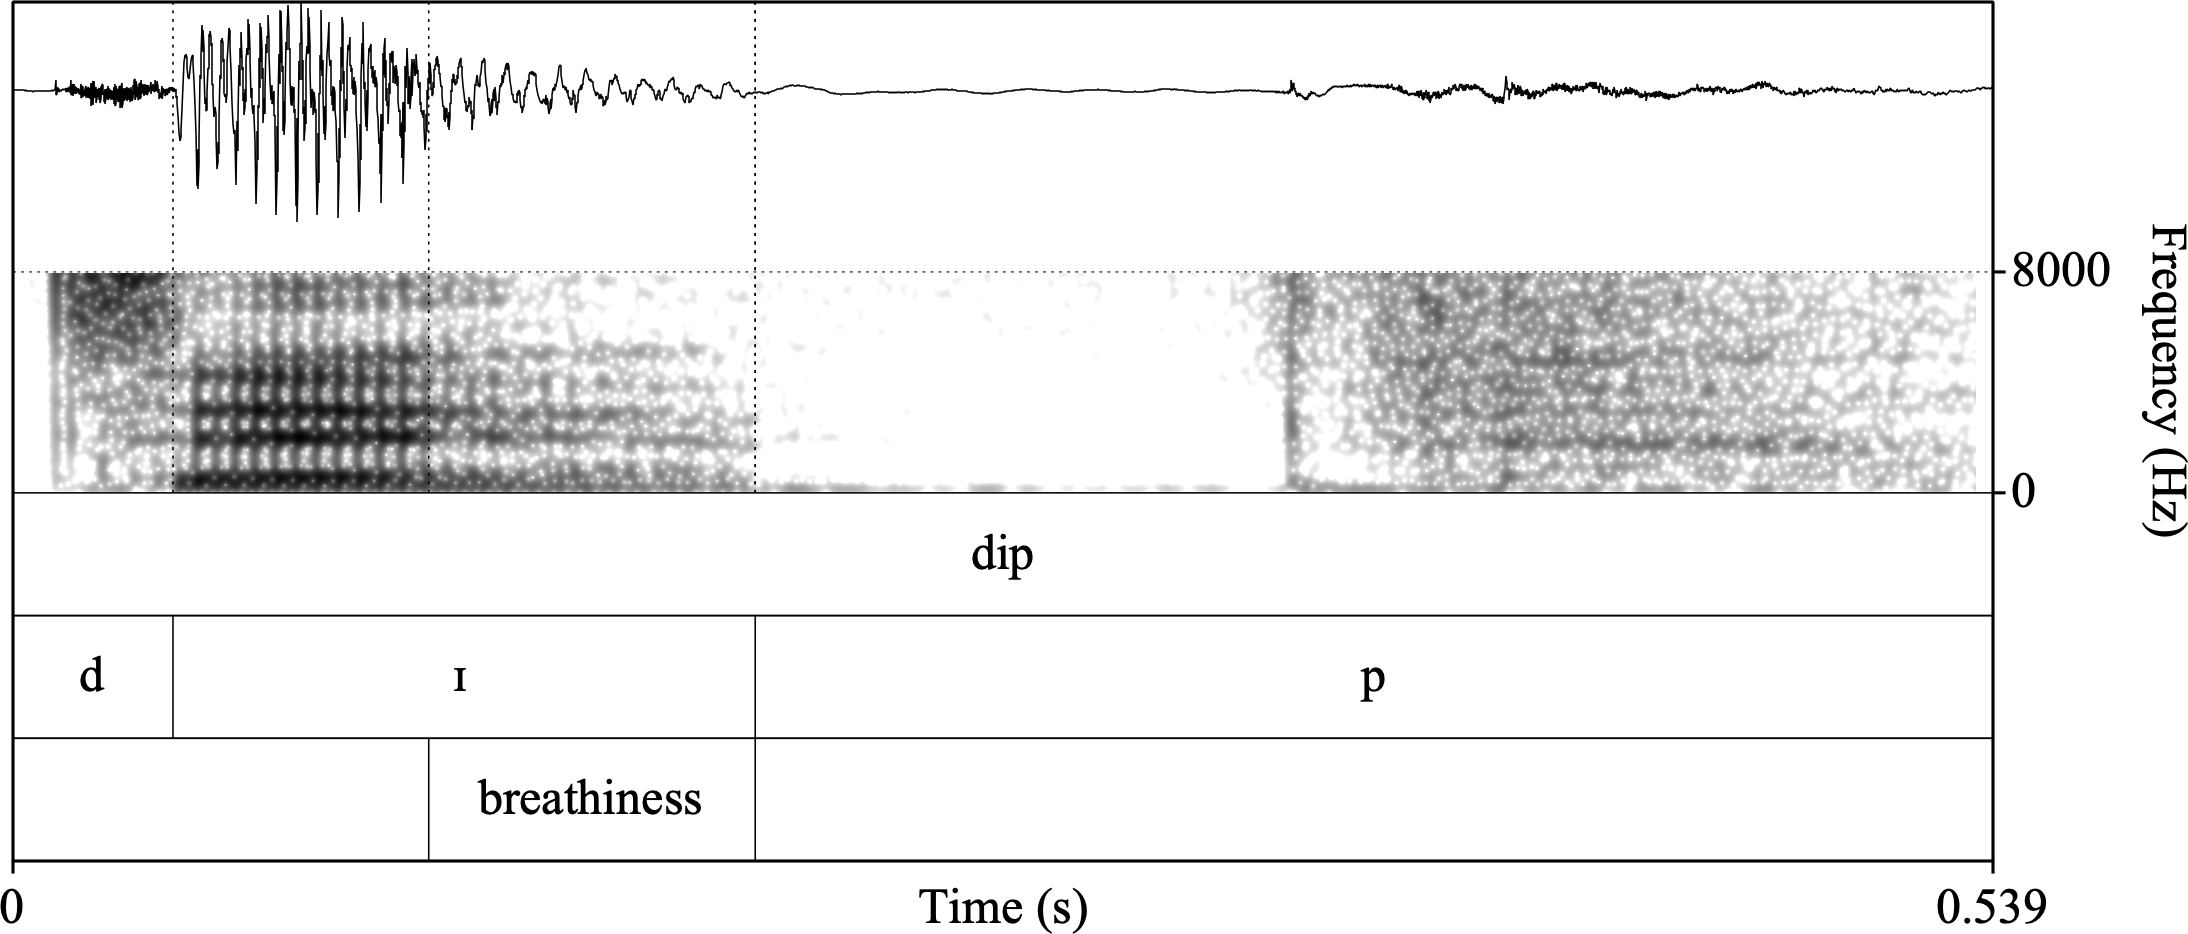
\includegraphics[width=\textwidth]{figures/Hejna-img004.png}
\caption{\label{fig:hejna:4} Pre-aspiration realised as local breathiness in the word \textit{dip}, as produced by a speaker of Welsh English. See \citet{Hejná2015, Hejná2016a, Hejná2016b} for more details}
\end{figure}

In addition, \citet[185, 373, 393]{Chasaide1985} has demonstrated that local breathiness can cue a contrast between an aspirated and an unaspirated plosive. This being the case, should cases that show local breathiness but no voiceless pre\hyp aspiration not be considered cases of pre\hyp aspiration as well? Even fewer researchers have commented on locally restricted breathiness (e.g. as a correlate of a fortis-lenis plosive contrast) than on voiceless pre-aspiration. A notable example is a study by \citet[310--315]{ChasaideGobl1993}, in which the authors report local breathiness in vowels preceding fortis obstruents in Swedish, Italian, and variably in English, but not in German and French. Researchers have discussed cases of contrastive breathiness (e.g. \cites[132]{Maddieson1984}[57--58, 317]{LadefogedMaddieson1996}), but this tends to be the case with vocalic and consonantal sonorants. In case of plosives, this is an aspect discussed for the release phase rather than the pre-closure phase. The question is how widespread local breathiness might be in the absence of voiceless aspiration in contexts which have been traditionally associated with pre-aspiration. A phenomenon such as local breathiness might be very easy to miss in the data. Some of the more general reasons for this are discussed in \sectref{sec:hejna:4.3}.

\section{But is pre-aspiration phonologically relevant?}\label{sec:hejna:3}
When the rarity of pre\hyp aspiration is discussed, it is frequently done through the lens of phonology: phonological pre\hyp aspiration is “an extremely rare phonological feature” (\citealt{Clayton2010}: iii) and it is rarely contrastive (e.g. \citealt{LadefogedMaddieson1996}: 70). More specifically, \citet[70]{LadefogedMaddieson1996} list Icelandic, Faroese, Scottish Gaelic, and Lule Sámi as languages with contrastive pre\hyp aspiration “on the surface level”. They further add that the phenomenon “is said to occur in Amerindian languages, such as the Algonquian language Ojibwa […] and the Arawakan language Guajiro” (\citeyear[72]{LadefogedMaddieson1996}). Four (plus) languages certainly do not present a particularly staggering number. However, we need to ask how contrastiveness and phonological relevance are established. These issues are discussed below.


\subsection{“Normative” pre-aspiration}\label{sec:hejna:3.1}

The literature available on pre\hyp aspiration leaves the reader with the impression that pre\hyp aspiration is seen as relevant if it is phonological, and that it is phonological only if it is contrastive. It also seems that in order to be seen as contrastive, pre\hyp aspiration needs to function as a primary (perceptual) cue to a contrast and as the most important – if not the sole – (production) correlate of the contrast in question. For instance, \citet{LadefogedMaddieson1996} make the following statements: 

\begin{quote}
Despite its importance in specifying the phonetic characteristics of some languages, we do not know of any language in which it is necessary to regard pre\hyp aspiration as a feature required for distinguishing underlying forms. \hfill\hbox{(\citeyear[73]{LadefogedMaddieson1996})}
\end{quote}

\begin{quote}
Pre-aspiration has been put at the bottom of the chart because it probably never forms the basis for contrasts among underlying forms.\hfill\hbox{(\citeyear[99]{LadefogedMaddieson1996})}
\end{quote}

The issue at hand is complicated by a very wide range of theoretical approaches available for the phonological analyses of contrasts. The first challenge to be encountered in the literature on pre\hyp aspiration is an assumption that only obligatory pre\hyp aspiration can be phonologically relevant.

For example, in his PhD thesis, \citet{Helgason2002} introduces a dichotomy of “normative” and “non-normative” pre-aspiration, adopted also by other scholars working on pre\hyp aspiration (e.g. \citealt{Morris2010}, among others). This dichotomy is nevertheless defined in two different ways in different works by Helgason.\footnote{The two different definitions are also found within his PhD thesis itself.} \textcites[1854]{Helgason1999}[8]{Helgason2002} defines normative pre\hyp aspiration as phonologically conditioned and obligatory. Importantly, “phonologically conditioned” and “obligatory” are put on par in this definition. However, an obligatory application of a phenomenon is not a precondition for its phonological relevance, since phonological rules can be variable (and phonetic rules can be obligatory, as one of the reviewers notes). Furthermore, it is not clear what rate of application should be considered obligatory pre-aspiration.

The second definition is linked to the consistent rate of application within a speaker community \citep[21]{Helgason2002}. If all speakers within a community pre-aspirated, for instance, 33\% of the times in the same contexts, this would fall within the category of “normative pre-aspiration” because we find a consistent rate of application across speakers. Most researchers adopting the normative and non-normative dichotomy use the second definition.

If we adopt the first criterion of pre\hyp aspiration being phonological only if applying obligatorily, it is perhaps not particularly surprising that the conclusion seems to be that pre\hyp aspiration is not phonologically relevant. This assumption nevertheless strikes me as somewhat misguided, because pre\hyp aspiration can function as a correlate and/or a cue to a range of contrasts, the most frequently discussed of which are the fortis-lenis contrast and the quantity contrasts, reviewed in \sectref{sec:hejna:3.3}. Before inspecting the literature on pre\hyp aspiration as a correlate of and/or a cue to a phonological contrast, we first need to briefly note on the phonological relationship between pre\hyp aspiration and post-aspiration (\sectref{sec:hejna:3.2}).

\subsection{Pre-aspiration does not contrast with post-aspiration}\label{sec:hejna:3.2}

As one of the reviewers points out, pre\hyp aspiration never contrasts with post-aspiration: aspiration is contrastive, rather than pre- or post-aspiration as such. It has been claimed that pre- and post-aspiration do not contrast with one another due to reasons related to prosodic licensing and sonority hierarchy and due to perceptual motivations (e.g. \cites[90--91, 94, 98, 101--103]{Blevins2004}[327]{GolstonKehrein1998}{GolstonKehrein2013}[Chapter 3]{Kehrein2002}{KehreinGolston2004}; see also \sectref{sec:hejna:4.1}). As such, pre\hyp aspiration and post-aspiration have been assumed to have identical phonological representations by a number of scholars (e.g. \citealt{Blevins2004}: 94). At least one exception to this typological generalisation might be Huautla Mazatec, which has been claimed to contrast pre- and post-aspirated word-initial obstruents on surface \citep{Steriade1994}. \citet{GolstonKehrein1998} nevertheless present an account whereby “pre-aspiration [has been] reanalyzed out of Mazatec phonology” (\citeyear[327]{GolstonKehrein1998}), which means that “there is no need to contrast [ht] and [th] in Huautla” (\citeyear[324]{GolstonKehrein1998}).

As \citet[94]{Blevins2004} states, however, “this phonetic difference [between post-aspirated and pre-aspirated stops] appears to determine the general sound patterns of aspirated stops both within and across languages”. Indeed, although \citet[327]{KehreinGolston2004} and \citet{Kehrein2002} argue that pre\hyp aspiration and post-aspiration are phonologically indistinguishable, they also fully acknowledge the fact that the two can be very distinct phonetically. Apart from the relevance of the distinction between pre\hyp aspiration and post-aspiration to typologists, the fact nevertheless remains that pre\hyp aspiration and post-aspiration can contrast with other properties of speech, such as the lack of pre\hyp aspiration and post-aspiration, respectively. This, then, renders them potentially contrastive, and this is the subject of Sections \ref{sec:hejna:3.3}--\ref{sec:hejna:3.4}.

\subsection{Fortis-lenis and quantity contrasts}\label{sec:hejna:3.3}

The categories “fortis” and “lenis” are used here for purely practical reasons, in line with \citet[105]{Chasaide1985}, “as convenient phonological terms to avoid the potentially confusing situation where one speaks of voiceless voiced stops, i.e. phonologically voiced stops with no phonetic voicing. The fortis/lenis labels are in no way intended to imply that either stop series is characterised by tense or lax qualities” (\citeyear[105]{Chasaide1985}). Namely, “fortis” is used in this chapter to cover consonants such as the English obstruents /p, t, k, f, θ, s, ʃ, tʃ/ and “lenis” to cover consonants such as the English obstruents /b, d, g, v, ð, z, ʒ, dʒ/.\footnote{This then differs from the definition of the fortis-lenis contrast as proposed by \citet{Trubetzkoy1939}.}

In terms of phonological contrasts, pre\hyp aspiration has been most often discussed in terms of its potential role in the fortis-lenis contrast of plosives (e.g. \mbox{/p, t, c, k/} vs. /b, d, ɟ, g/). As already mentioned, \citet[70]{LadefogedMaddieson1996} list four languages as having contrastive pre-aspiration: Icelandic, Faroese, Scottish Gaelic, and Lule Sámi. The importance of this source cannot be overstated. Research conducted since then has found that pre\hyp aspiration is a robust correlate of a fortis-lenis contrast in more languages, which belong to eleven language families (Afro-Asiatic, Algic, Arawakan, Austronesian, Indo-European, Mongolic-Khitan, Otomanguean, Tucanoan, Uralic, Uto-Aztecan, and two isolates: Urarina and Yuchi). The presence of such research is marked in the final column of Tables 1--19 in the Appendix. Yet, as we will see in \sectref{sec:hejna:5}, various typological databases do not reflect this recent research on pre-aspiration.

Furthermore, apart from the plosive context, pre\hyp aspiration has also been documented as a correlate of the fortis-lenis contrast in fricatives in Scottish Standard English (\citealt{GordeevaScobbie2010,GordeevaScobbie2013}), Forest Nenets \citep{Salminen2007}, and Wanano \citep[50--51]{Stenzel2004}. 

Most studies which look into whether or not pre\hyp aspiration may function as a correlate of the fortis-lenis contrast do so by looking into whether pre\hyp aspiration is present in one of the two series and, if so, how frequently. However, some of the production studies of the phenomenon intriguingly show that it is not necessarily the presence and absence of pre\hyp aspiration which distinguishes the fortis and lenis plosives but its duration (longer in one series than in the other, comparably to VOT, cf. \citealt{DiCanio2012, MorrisHejná2020, NanceStuart-Smith2013}). Thus, \citet{DiCanio2012} reports two phonological groups which both contain pre-aspiration, but this pre\hyp aspiration is consistently longer in one of the two series than the other. It is rare for studies that investigate whether or not pre\hyp aspiration functions as a correlate of a contrast to compare pre\hyp aspiration with other potentially relevant correlates of the same contrast. \citet{Engstrand1987} presents one of these not very frequent studies. Comparing pre\hyp aspiration and VOT, \citet[103]{Engstrand1987} explicitly states that, unlike pre-aspiration, VOT is irrelevant in the word-medial contrast of fortis-lenis in Lule Sámi.

We might wonder to what extent pre\hyp aspiration functions also as a perceptual cue to the fortis-lenis contrast in the languages in question. Unfortunately, the research on this topic is considerably limited. That pre\hyp aspiration can function as a cue to a fortis-lenis contrast has been shown for English (\citealt{HejnáKimper2019}), Icelandic (\citealt{Chasaide1985}: Ch. 5), Norwegian (\citealt{Dommelen1999}), Scottish Gaelic (\cites{Clayton2010}[Ch. 5]{Chasaide1985}), and Swedish (\citealt{HelgasonRingen2008}: 625). Interestingly, \citet[435]{Chasaide1985} shows that pre\hyp aspiration can cue the contrast in Icelandic and Scottish Gaelic at much shorter durations than what her production data might suggest. The exact durations and their perception as pre-aspirated however depend on a range of factors in her study, including the amplitude of pre\hyp aspiration and the duration of the closure of the plosive.\footnote{Ní Chasaide only investigated plosives.} \citet{HejnáKimper2019} show that discrimination and identification tasks yield somewhat different results. Voiceless pre\hyp aspiration duration of 80\,ms was needed to increase the identification of a pre-aspirated plosive as fortis. On the other hand, in the discrimination task, the listeners could reliably tell a difference between pre\hyp aspiration durations of 0\,ms and 20\,ms, 20\,ms and 40\,ms, and 40\,ms and 60\,ms, but longer durations did not lead to higher “fortis” responses.

Discussions of the fortis-lenis contrast also include considerations of quantity contrasts, as the two can be very closely intertwined. For instance, \citet{DiCanio2012} presents the case of San Martín Itunyoso Trique (Otomanguean) and argues that what has been approached as a fortis-lenis contrast should instead be considered a singleton-geminate contrast. Another intriguing case is presented in \citegen{wretlingetal2002} analysis of pre\hyp aspiration in Swedish dialects. The fortis/geminate obstruents are consistently associated with (more frequent) pre-aspiration. In addition, discussions as to whether pre\hyp aspiration is part of the vowel or the consonant might also have implications for the analyses of vowel length. Pre-aspiration has been documented as a correlate of quantity contrasts in languages such as Icelandic and Lule Sámi. Most frequently, this involves a singleton-geminate contrast (e.g. Blackfoot – \citealt{ReisSilva2008}; Icelandic – \citealt{Silverman2003}; Italian – \citealt{Stevens2010, StevensReubold2014}; for the intriguing case of Southern Paiute, see \citealt{Silverman2003}: 587--588). Lule Sámi and Skolt Sámi present very interesting cases where three quantity degrees correlate with the presence and duration of pre\hyp aspiration (\citealt{Engstrand1987, McRobbie-Utasi2003}). 

Some perceptual evidence has been provided on the role of pre\hyp aspiration in quantity contrasts. The reader is referred to \textcite[Ch. 3]{Helgason2002}, \textcite{Pind1996Rate, Pind1996RateQuantity} and \citet{StevensReubold2014}.

\subsection{Other contrasts}\label{sec:hejna:3.4}

Varieties of English, such as Manchester English (\citealt{HejnáScanlon2015}) and Scottish Standard English (\citealt{GordeevaScobbie2013}), also show that pre\hyp aspiration may be a correlate of manner contrasts. If pre\hyp aspiration consistently applies in word-final fortis fricatives (e.g., \textit{mass} [maʰs]) and (pre-)glottalisation consistently applies in word-final fortis plosives (e.g. \textit{mat} [maˀtˢ]), pre\hyp aspiration can be said to function as one of the correlates of the /s/ -- /t/ contrast. Depending on the analysis, this might also be the case in Menominee \citep{Gathercole1983}.

Another type of contrast is mentioned by \citet[590]{Silverman2003}, who discusses pre\hyp aspiration in Huautla Mazatec, in which the cluster [sk] contrasts with [ʰk]. This is not the case for /t/, as there is no cluster /st/ in the language. Such type of a contrast involving pre\hyp aspiration would belong to the contrasts of the place of articulation.

Finally, in some languages (e.g. \citealt{Silverman2003}: 589, who mentions Hopi, Tarascan, Scandinavian languages, Scottish Gaelic, and Chamicuro), pre\hyp aspiration is restricted to stressed syllables. In this case, pre\hyp aspiration is involved in the complex web of correlates of stress and prominence.

\subsection{Other criteria of phonological relevance}\label{sec:hejna:3.5}

\textcites[Ch. 4]{Hejná2015}{Hejná2019} discusses criteria which can be used to establish whether pre\hyp aspiration is conditioned phonologically in a language even beyond the most widely established diagnostic of contrastiveness. To summarise, pre\hyp aspiration in Aberystwyth English (i.e. Welsh English) shows variation which cannot be explained solely by phonetic (or social) factors. Firstly, it is phonological rather than phonetic vowel height (as in \textit{kit} /kɪt/ vs \textit{cat} /kat/) which predicts the duration of pre\hyp aspiration in this data. Namely, while pre\hyp aspiration is sensitive to the phonemes with different (phonological) height, it is not sensitive to F1 (the acoustic correlate of height) within these vowel phoneme categories. Secondly, phonetic vowel duration positively correlates with the duration of pre-aspiration, but this is only the case in phonologically short (or lax) vowels. A negative correlation is, in turn, found in phonologically long (or tense) vowels.\footnote{The strength of these correlations is speaker-specific.} 

Thirdly, the duration of pre\hyp aspiration consistently shows a bimodal distribution, which has been used to diagnose phonological relevance (e.g. \citealt{Hejná2015}: Chapter 4 for an overview). In case of Aberystwyth English pre-aspiration, the phenomenon reveals the presence of two categories: some words have no pre\hyp aspiration (0\,ms) while others have pre\hyp aspiration of durations which form a mode, or indeed a category, of their own (clustered around {\textasciitilde}20--70\,ms, depending on the speaker). These two categories remain present even when a relatively wide range of segmental and prosodic factors is controlled for, and, therefore, cannot be explained by the influence of other phonetic factors.

Although determining the phonological status of pre\hyp aspiration is essential in the discussions of its typological features (or distribution), I would like to conclude this section by pointing out the value of phonetic and sociolinguistic (more below) descriptions of pre-aspiration, which are equally important for a comprehensive understanding of its typology (e.g. \citealt{ChoLadefoged1999, MoisikEtAl2022, MorrisHejná2020}). The implication in typological studies seems to be that unless pre\hyp aspiration is phonological, it may not be worth discussing or even acknowledging at all, which possibly underrates its presence in the world’s languages. The discussions brought to light here are ultimately linked to those surrounding the phonetics-phonology interface, and to what \textcitetv{chapters/02_Iosad} refers to as analytical indeterminacy.

Finally, although social aspects of speech communities may not be seen as having a place in typological descriptions (as inferred from a number of typological discussions of pre-aspiration), sociophonetic work can offer cross-linguistically relevant understanding of the conditioning of specific phenomena, also but not only because sociophonetics has to address the biology of the speakers. Regarding pre\hyp aspiration more specifically, different groups of pre-aspirating speakers can produce different frequencies, durations, and noisiness levels of pre\hyp aspiration (e.g. \citealt{Clayton2017, Hejná2021, HejnáEtAl2020, HejnáEtAl2021, Morris2010, MorrisHejná2020, NanceStuart-Smith2013}). Age and sex/gender have been shown to condition pre\hyp aspiration (see \citealt{Hejná2015, MorrisHejná2020} for overviews), and research is yet to show to what extent these patterns are due to biological age and sex, social age and gender, or a mixture of the biological and the social.

\section{Should pre\hyp aspiration be rare and why?}\label{sec:hejna:4}
\subsection{Difficult to perceive?} \label{sec:hejna:4.1}

The main reason put forward to account for the rarity of pre\hyp aspiration in the world’s languages is that it is difficult to perceive. In his chapter arguing for the importance of the hearer (or the listener) in phonetics, \citet[7]{Bladon1986} states that, in the case of pre-aspiration, “[i]t would be hard to imagine a speech pattern less favourably designed for the hearer”, and “given that preaspiration suffers from an accumulation of auditory handicaps, it would not be a risky prediction that languages would rarely make use of this auditory-phonetic dinosaur”.\footnote{It is \citet[19]{Clayton2010} who first drew attention to Bladon’s claims about the perception of the phenomenon in work focusing primarily on pre-aspiration.} As discussed in \sectref{sec:hejna:2.2}, \citet{Silverman2003} explains the fact that pre\hyp aspiration is often accompanied by oral frication (pre-spirantisation) or substituted by it because this makes it perceptually more audible. The potentially weak perceptibility of pre\hyp aspiration is what \citet[87]{Clayton2010} has titled the Perceptual Inferiority Hypothesis. The overall explanation put forward in his work maintains that post-aspiration is easier to perceive than pre\hyp aspiration because “it is easier to hear the onset of a stimulus than its end” (\citealt{Clayton2010}: 88, paraphrasing \citealt{Bladon1986}). A plosive burst is in itself an acoustically and perceptually more salient phenomenon than a segmental offset. Kingston labels this “the problem of pre-aspirates” (\citealt{Kingston1990}: 410, also \citealt{Silverman2003}: 593--594).

As discussed in \sectref{sec:hejna:3}, however, there are too few experimental studies directly testing the perceptibility of pre-aspiration. Firstly, one can consider the literature presented in the discussion of pre\hyp aspiration as a correlate of a phonological contrast (\sectref{sec:hejna:3}), which fairly consistently shows that pre\hyp aspiration does function as a correlate of a contrast where researchers specifically investigate this possibility. This being the case, we may wonder why pre\hyp aspiration should serve as a correlate of any phonological contrast if it is not perceptible as a cue of the contrast in question.

The most direct test is presented by \citet[95--107]{Clayton2010}. He uses L1 English, Polish, and Scottish Gaelic listeners in his discrimination experiment, in which initial (fortis/lenis) plosives are distinguished by post-aspiration, and the medial and final ones by pre-aspiration. Crucially, this experiment uses Scottish Gaelic words for all participants. Both post- and pre\hyp aspiration have long been established as correlates of the fortis-lenis contrast in the language (e.g. \citealt{NanceStuart-Smith2013}). It is not surprising, then, that the Scottish Gaelic listeners performed the best. Interestingly, their confusion rate was the highest in the final position. The English listeners performed better with initial post-aspiration than medial pre\hyp aspiration and the worst with final pre-aspiration. On the whole, their confusion rates were higher than is the case for the Scottish Gaelic listeners. Finally, the Polish listeners showed higher confusion rates for initial post-aspiration than either the Scottish Gaelic or the English listeners. However, they performed better in cases of medial and final pre\hyp aspiration in comparison with the English listeners, and in the medial position their confusion rates were very close to those of the Scottish Gaelic listeners. Clayton interprets these results to indicate that the Perceptual Inferiority Hypothesis is not confirmed, and proposes instead that the answer to why pre\hyp aspiration is rare lies in the availability of historical precursors (see \sectref{sec:hejna:4.2}).

However, more perceptual experiments are needed, including those in which post-aspiration and pre\hyp aspiration are compared in the same prosodic position.\footnote{One of the reviewers notes that, according to the proposals by \textcite{KehreinGolston2004, GolstonKehrein2013}, “that won’t happen because the [pre-aspiration and post-aspiration] distinction is usually prosodically determined”. Irrespective of what “that” refers to exactly here, while there is no doubt that pre\hyp aspiration and post-aspiration show strong distributional differences determined by prosody, including both in the same prosodic condition nonetheless remains essential to test the claims put forward about the disadvantaged status of pre\hyp aspiration as a cue.}

\subsection{Difficult to innovate?} \label{sec:hejna:4.2}

Rather than being difficult to perceive, Clayton proposes instead that the main reasons for the rarity of pre-aspirated plosives are the low rates of innovation and the competition with multiple rephonologisation candidates rather than the low transmission rates (\citeyear[86--87]{Clayton2010}). More specifically, pre\hyp aspiration is rare because the conditions under which it innovates are restricted. The number of paths of innovation that lead to pre\hyp aspiration is a more likely explanation than perceptual biases. This explanation is also in line with the observation that pre\hyp aspiration has been fairly stable diachronically in, for instance, Nordic languages.\footnote{\citet{Clayton2010} uses the term “Nordic languages”, which is what this section of the chapter therefore uses as well.} Five cross-linguistically attested antecedents of pre\hyp aspiration have been proposed:

\begin{enumerate}
\item geminates: pre\hyp aspiration has developed from originally degeminate consonants in some languages (e.g. Nordic languages, Scottish Gaelic, Sámi, Forest Nenets, Bora; cf. \citealt{Clayton2010}: Chs. 2\&3, and Sect. 3.1.2 in particular);
\item nasal-stop clusters: nasals can give rise to pre\hyp aspiration in clusters (Central Algonquian languages, possibly some instances in Nordic languages, Hopi; cf. \citealt{Clayton2010}: Chs. 2\&3, and Sect. 3.1.2 in particular);
\item spontaneous appearance in singleton voiceless stops (\citealt{Clayton2010}: Chapter 3);
\item borrowing/contact \citep[61--62]{Helgason2002};
\item /s/-stop clusters (\citealt{Silverman2003}: 593, also \citealt{Suzuki2011}).
\end{enumerate}

\citet{Clayton2010} adds an important detail: pre\hyp aspiration “tends to occur in languages featuring two stop series that contrast through aspiration, not voicing” (\citeyear[33]{Clayton2010}). This is echoed in \citet[e.g. 42]{Hejná2015}, who discusses local breathiness as a potential diachronic step towards the development of voiceless pre\hyp aspiration through the anticipation of the laryngeal abduction associated with post-aspiration.

In addition, \citet[242]{Hejná2015} suggests that pre\hyp aspiration is more likely to innovate in stressed syllables. While \citet[42]{Hejná2015} also mentions the possibility of pre\hyp aspiration developing from pre-glottalised consonants, this suggestion is, at this point, too speculative (see also \sectref{sec:hejna:2.5} above and \citealt{Hejná2023}).

In addition to drawing attention to the number of phonetic precursors, \citet[70]{Clayton2010} also mentions the importance of “the abundance of antecedent structures” – in other words, a question of how common the precursors themselves are. In order to understand whether the rarity of pre\hyp aspiration could be explained through the low abundance of the necessary precursors, it first needs to be established how rare the precursors are. Is post-aspiration more common than pre\hyp aspiration because the contexts under which pre\hyp aspiration is likely to innovate are more restricted than those for post-aspiration, for instance? Considering the precursors listed above, at least the following, more specific, questions should be explored in future research:

\begin{enumerate}
\item How many languages have phonetically voiceless obstruents, and ideally post-aspirated ones, either in a coda (e.g. Welsh English \textit{mat} [maʰtˢ]) and/or in a foot-medial syllabic onset (e.g. Welsh English \textit{matter} [maʰtˢə])?
\item How many languages have clusters of /s/ and voiceless plosives, and ideally in post-tonic environments?
\item How many languages have geminates, and ideally post-tonic ones?
\item How many languages have clusters of nasals and voiceless plosives, and ideally in post-tonic environments?
\end{enumerate}

The next section focuses on the last category of reasons which might lead to the conclusions that pre\hyp aspiration is cross-linguistically rare.

\subsection{The limitations of the analyst}\label{sec:hejna:4.3}

In addition to what has been discussed in \sectref{sec:hejna:4.1} and \sectref{sec:hejna:4.2}, there are also other aspects that may explain the rarity of pre-aspiration. These are related to the limitations of the analyst.

\subsubsection{Quality of the data}

Firstly, pre\hyp aspiration is often of low-amplitude and occurs following a highly sonorous segment. Because pre\hyp aspiration often includes glottally produced low-intensity friction, it is particularly prone to being acoustically (i.e., both visually and audibly) masked in the acoustic signal. This might therefore happen not only due to the acoustic properties of pre-aspiration, but also due to the types of segmental combinations in which pre\hyp aspiration is found. I limit the discussion here only to acoustic echoing in the sequences of vowels and phonetically voiceless obstruents (a prototypical context for pre-aspiration). A sonorous segment which is echoed into what might be a period of pre\hyp aspiration and\slash or closure of a plosive might mask the potential presence of pre\hyp aspiration in the acoustic signal. Figures \ref{fig:hejna:5}--\ref{fig:hejna:6} show such instances of echoing.

  
\begin{figure}
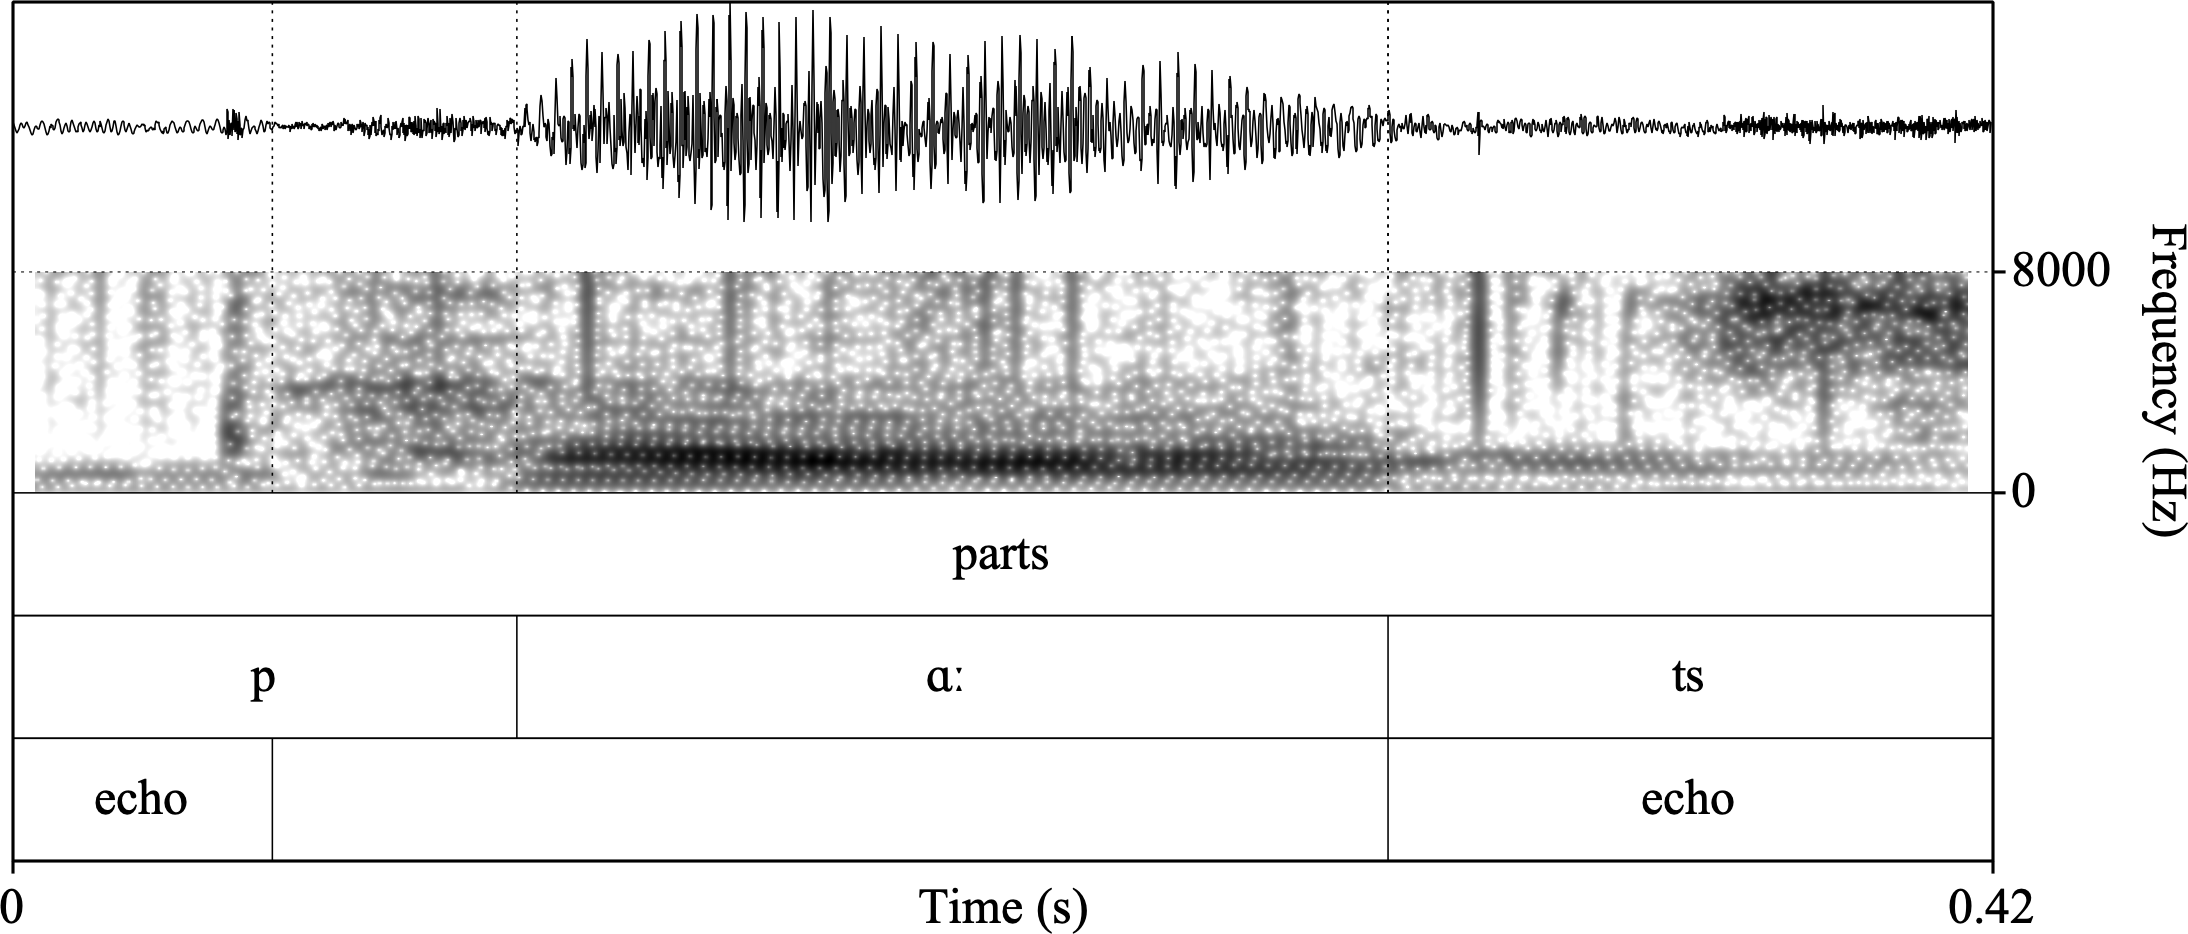
\includegraphics[width=\textwidth]{figures/Hejna-img005.png}
\caption{\label{fig:hejna:5}Example of acoustic echoing. The word \textit{parts}, as produced by Queen Elizabeth II in her 1952 Christmas speech. The segmentation of the boundary between /pɑː/ and /ts/ is also approximate as a result. Data kindly provided by Jonathan Harrington}
\end{figure}
  
\begin{figure}
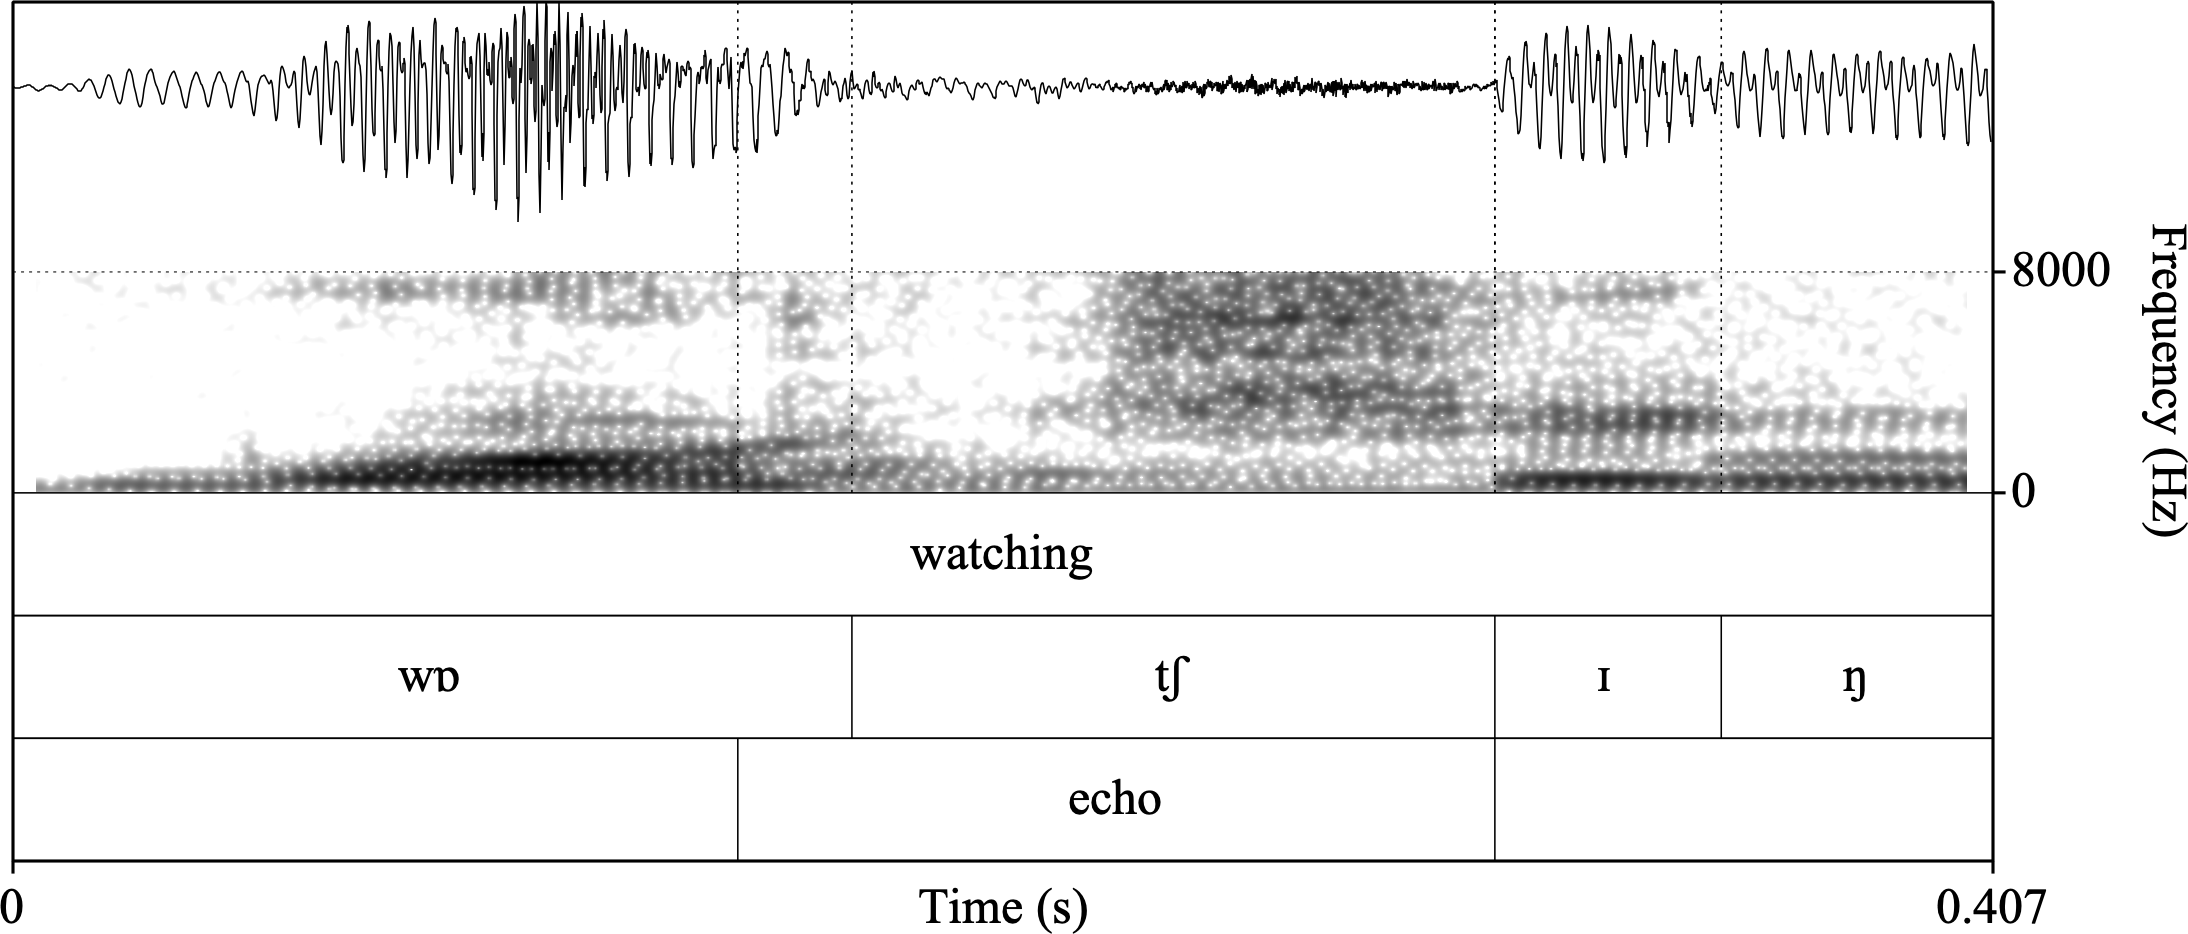
\includegraphics[width=\textwidth]{figures/Hejna-img006.png}
\caption{\label{fig:hejna:6}Example of acoustic echoing. The word \textit{watching}, as produced by Queen Elizabeth II in her 1988 Christmas speech. The segmentation of the boundary between /wɒ/ and /tʃ/ is also approximate as a result. Data kindly provided by Jonathan Harrington. The message can also be accessed here: \url{https://www.youtube.com/watch?v=LvpFJesl5hE}}
\end{figure}

Figures \ref{fig:hejna:5}--\ref{fig:hejna:6} show examples of ambiguously pre-aspirated tokens from Queen Elisabeth II’s Christmas broadcasts, which are of fairly good quality but not good enough for the reliable identification of what may be short and weak pre\hyp aspiration in various places. In Figures 5--6, the ambiguous case of pre\hyp aspiration appears in a sequence of a vowel and a plosive/affricate (/ɑːt/ in \textit{parts} and /ɒtʃ/ in \textit{watching}). The vowel is necessarily produced with a considerably higher intensity than potential pre-aspiration. If echoing occurs, it follows the original (unechoed) vowel, exactly where we would expect to find pre-aspiration. The consistency and the magnitude of the echoing depend on a range of factors. These include not only the quality of the equipment and its stable placement, but also the positioning and movements of the speakers, and the general acoustics of the surroundings in which the data is obtained

\subsubsection{Confirmation bias}

Biases of researchers are another challenge we have to tackle as analysts (including our own biases). The scholarly literature available, just like any type of text, presents us with specific discourses. As a result of such discourses, researchers may not even look for pre\hyp aspiration in their data a priori, especially if it is known and frequently discussed as a rare phenomenon. Not expecting pre\hyp aspiration a priori is one form of confirmation bias (see \citealt{Klayman1995} for a general overview). However, researchers may also fail to detect pre\hyp aspiration if they deem it phonologically irrelevant.\footnote{Another case in point is voicing in obstruents. One of the reviewers commented on \figref{fig:hejna:1}, which originally included the /b/ of \textit{bat}. The phoneme /b/ is partially voiced: partial voicing functions as one of the correlates of the fortis-lenis plosive contrast in Aberystwyth English (e.g. \citealt{Hejná2016b}). The reviewer’s suggestion was to “chop [this voicing] off as irrelevant to [b] which is probably just a voiceless (unasp) stop” and likely “part of something that precedes [the /b/], or \emph{ambient noise}” (emphasis mine). The reason why this voicing should not be “chopped off” is because it consistently occurs in the lenis series – and not in the fortis series – in the variety in question, and in data where no acoustic echoing is present.} Nonetheless, whether or not a phenomenon is contrastive does not mean that speakers do not employ it for various functions. Yet, frequent claims about the rarity of pre\hyp aspiration (as contrastive) can easily lead one to expect it to be rare even in data which may be of interest to researchers who are not necessarily concerned with questions of contrastiveness. The issue of a potential confirmation bias is also linked to the bias raised by \citet{Maddieson2021}: “Familiarity with dominant languages can distort ideas about the phonological patterns of language in general and lead the linguistic community away from valuing all languages equally”. We could easily substitute “languages” with “phenomena” in this quotation.

\subsubsection{Language skills of the analyst}

Furthermore, it is also likely that some languages are documented as pre-as\-pi\-ra\-ting in literature which is available only in the languages in which most researchers are not sufficiently proficient. To give one example, my former student Wenyu Guo, an L1 speaker of Chinese, brought my attention to work on pre\hyp aspiration in Chahar (Mongolic) by Qascimeg (Hāsīqímùgé) (\citeyear{Qascimeg2008}), available in Chinese only.

\section{How rare is pre-aspiration?}\label{sec:hejna:5}

Quantifying occurrences of pre\hyp aspiration in the languages of the world is far from straightforward, as should have become apparent by this point. Pre-as\-pi\-ra\-tion presents us with several thorny issues of a diverse nature. While we are extremely fortunate to have open-access databases, such as UPSID (based on 451 languages, \citealt{MaddiesonPrecoda1990}) and its follower LAPSyD (676 languages, \citealt{MaddiesonEtAl2016}), these databases do not present the level of detail which is needed in case of pre-aspiration.

For example, when we use LAPSyD, the “search for contrast” function can be employed. If pre\hyp aspiration is selected, 2 out of 676 languages included in the database are listed as containing contrastive pre\hyp aspiration (for plosives and affricates), in contrast to 109 languages listed as having post-aspiration. The two pre-aspirating languages are Tunica (/p, t, k, tʃ/) and Hopi (/p, t, k, q, kw, ts/). The database also offers a Boolean operator function, which provides us with the same results. The two pre-aspirating languages present 0.3\% of the database, which is considerably lower than the percentage of post-aspirating languages reported in the database (24.2\%).\footnote{Readers like myself might be surprised that post-aspiration – considered to be quite widespread – is still represented by only 24.2\% of languages.} Anyone familiar with the recent research on pre\hyp aspiration would nevertheless be hesitant to draw solid conclusions about the rarity of pre\hyp aspiration in the languages of the world based on LAPSyD, because it seems to be heavily underrepresented in this resource.

Based on the evidence gathered in this chapter, it can be concluded that pre\hyp aspiration has been reported in at least 19 language families, and {\textasciitilde}84 languages,\footnote{See \textcitetv{chapters/02_Iosad}, for pre\hyp aspiration and phonological areality.} bearing in mind that the discussion of whether all of these languages do have pre\hyp aspiration (as opposed to, for example, clusters with /h/) and whether this pre\hyp aspiration is contrastive will depend on future research and the analyst’s biases and decisions about the criteria to be used. According to Glottolog 4.5 (\citealt{NordhoffHammarström2011}), there are 427 language families in the world, represented by 4,775 languages. Absolute counts of language families and those of individual languages/varieties are bound to be contentiously debated. Bearing this in mind, and bearing in mind that the number of 84 pre-aspirating languages is itself subject to contentious debates, we get a number of 4.45\% of the language families which have been documented to contain at least some more or less confirmed cases of pre-aspiration. As for the concrete languages, 84 amounts to 1.8\% of a total of 4,775.\footnote{This is a conservative number, which is ultimately linked to issues related to distinctions between dialects and languages.}

These numbers are rather low indeed, despite the lax approach to pre\hyp aspiration adopted here, which includes even the languages in which the presence of pre\hyp aspiration has been contested in one or more sources, so pre\hyp aspiration can indeed be considered to be a phonetic/phonological rarity. 

\section{Where does this leave us?}\label{sec:hejna:6}

This chapter started with the following questions related to pre-aspiration:

\begin{itemize}
\item RQ1: How is pre\hyp aspiration defined?
\item RQ2: Is pre\hyp aspiration rare?
\item RQ3: Why should(n’t) pre\hyp aspiration be rare?
\end{itemize}

As we could see, pre\hyp aspiration has been defined in many ways. Some of the definitions also include other phonetic and phonological phenomena related to pre\hyp aspiration such as pre-affrication, pre-spirantisation, debuccalisation of /s/, vowel devoicing, sonorant devoicing, and others. Some definitions – the most common ones – restrict pre\hyp aspiration to voiceless obstruents, while others extend the potential occurrence of the phenomenon also to sonorant consonants. From a diachronic perspective, many of these phenomena are often intertwined. On a synchronic level, the definition of pre\hyp aspiration as broad or narrow may depend on the analyst’s aims and the scope of intended research. Different approaches to the definition of the phenomena will necessarily impact our answer to RQs 2 and 3.

Regarding RQ2, the position taken in this chapter is that pre\hyp aspiration can be phonologically relevant in a range of ways. Even in cases when it is not, it may be subject to the conditioning by sociolinguistic factors in the few languages where those have been looked into. Ultimately, if we want to understand the maximal scope of the rarity of pre\hyp aspiration in the languages of the world, the cases of non-contrastive pre\hyp aspiration should also be taken into account.

In response to RQ3, I documented a range of cases where pre\hyp aspiration does contribute to the phonetic implementation of certain contrasts. I also discussed ways to diagnose the indirect phonological relevance. 

In addition, I touched upon several biases which likely contribute to seeing pre\hyp aspiration as a rare or very rare phenomenon. Those biases are related to the a priori expectations of researchers about the absence of pre\hyp aspiration and to the low quality of the acoustic data itself. Finally, structural prerequisites for pre\hyp aspiration were discussed in connection with the claimed rarity of the phenomenon.

In conclusion, I would like to invite the readers to join me and so many others in providing more information about pre\hyp aspiration so that we better understand this fascinating and complex phenomenon from a typological perspective. To help us in this endeavour, I formulate the following research questions and goals.

\begin{enumerate}
\item In order to understand what pre\hyp aspiration is and where it is, we also need to agree on what it is not. What are the differences between pre\hyp aspiration and vowel devoicing? Which languages have pre\hyp aspiration and which languages have vowel devoicing? Which languages have both? Why should at least some types of debuccalisation (not) be considered as sources of pre-aspiration? Why should some clusters but not others (not) be considered potential sources of pre-aspiration? How common is local breathiness occurring on its own, i.e. in the absence of voiceless glottal friction, in contexts typically associated with pre-aspiration?
\item Are pre-aspirated fricatives less common than post-aspirated fricatives, similarly to the situation observed in plosives?
\item How do we establish whether pre\hyp aspiration is phonological? Is pre\hyp aspiration a correlate of a contrast (not necessarily a fortis-lenis or a voicing contrast) in a language where it has been reported? Is it a cue to a contrast? If so, is it one of the primary and secondary correlates and cues? Is pre\hyp aspiration conditioned by phonetic factors or also phonological ones?
\item Should we report if pre\hyp aspiration is present only if we suspect that it is phonological (whatever that means to the researcher in question)? What are the social functions of pre-aspiration, and how diverse are these in pre-aspirating languages? Is pre\hyp aspiration subject to biological types of conditioning, and if so, what are these?
\item What are the spectral properties of pre\hyp aspiration in pre-aspirating languages? Do these relate to the spectral properties of the post-aspiration in the same language, if these have post-aspiration, and how exactly?
\item Which and how many languages of the world have the most common preconditions for pre\hyp aspiration to innovate? Which and how many languages have phonetically voiceless obstruents, and ideally post-aspirated ones, either in a coda (e.g. Welsh English \textit{mat} [maʰtˢ]) and/or in a foot-medial syllabic onset (e.g. Welsh English \textit{matter} [maʰtˢə])? Which and how many languages have clusters of /s/ and voiceless plosives, and ideally in the environments just described above? Which and how many languages have geminates, and ideally in the environments described above? Which and how many languages have clusters of nasals and voiceless plosives, ideally in the environments described above?
\item Once the numbers of languages with these environments are established, how do these fare with those where post-aspiration is found?
\end{enumerate}

Pre-aspiration comes out as rare based on the evidence available. However, it needs to be borne in mind that just because it is not reported to be present in a specific language, it may not be the case that it is not there. Absence of evidence does not equal evidence of absence. Undoubtedly, documenting evidence of absence might be a more challenging task, but one which is nonetheless important. Although pre\hyp aspiration may not be quite as rare as believed, the current literature nevertheless suggests that it takes its place next to other phenomena considered to be very rare, such as ejective fricatives.

\section*{Acknowledgements}

I would like to thank Cormac Anderson for his invitation to submit an abstract to the session “Rarities in phonetics and phonology: evolutionary, structural, typological and social dimensions” at the 50th Poznań Linguistics Meeting in 2021. Very important was also the encouragement I received from the PLM audience, and that of Cormac, Natalia Kuznetsova, Pavel Iosad, and Janet Watson in particular. I would also like to thank Ian Maddieson for a useful exchange of ideas on the many different things that one could put under the umbrella label of “pre-aspiration”. Natalia Kuznetsova has been incredibly instructive with her detailed feedback on the chapter and has my many very sincere thanks. Finally, I would like to thank Daniel Silverman for his fantastic 2003 paper on pre-aspiration.

\printbibliography[heading=subbibliography,notkeyword=this]

\begin{paperappendix}
  % ATTENTION: Diacritics on the following phonetic characters might have been lost during conversion: {'ɛ'}


\begin{table}
\begin{tabularx}{\textwidth}{@{}l@{}QQQl}
\lsptoprule
& Languoid & Reference & F/L contrast & Code\\
\midrule
 & San’ani Arabic & \citet{WatsonHeselwood2016} & \citet{WatsonHeselwood2016} for /t/ vs emphatic /ṭ/ & sana1295 / ayn\\
& Śḥerɛt/Jibbali & \citet{chapters/12_WatsonEtAl} & \citet{chapters/12_WatsonEtAl} & sheh1240 / shv\\
\lspbottomrule
\end{tabularx}
\caption{Afro-Asiatic languages reported to have pre-aspiration}
\label{tab:key:1}
\end{table}


\begin{table}
\begin{tabularx}{\textwidth}{@{}l@{}QQQl}
\lsptoprule
& Languoid & Reference & F/L contrast & Code\\
\midrule
  & Amuesha/Yanesha & \citet{Silverman2003} &  & yane1238 / ame\\
& Blackfoot &  \citet{ReisSilva2008} &  \citet{ReisSilva2008} & algo1256\\
& Plains Cree & \citet{Hewson1993} &  & plai1258 / crk\\
& proto-Algonquian & \citet{Hewson1993} &  & \\
& (Swampy) Cree & \citet{Silverman2003} &  & swam1239 / csw\\
& Eastern Ojibwa & \citet{Silverman2003} &  & east2542 / ojg\\
& Fox (Kickapoo) & \citet{Silverman2003}, \citet{Gathercole1983} & \citet{Gathercole1983}; ? \citep[586]{Silverman2003} & kick1244 / kic\\
& Menominee & \citet{Clayton2010} &  & meno1252 / mez\\
& Montagnais & \citet{chapters/17_Craioveanu} &  & mont1268 / moe\\
& Natick (Massachusee / Wampanoag) & \citet[30]{Hewson1993} &  & wamp1249 / wam\\
& Penobscot & \citet[30]{Hewson1993} &  & peno1243\\
\lspbottomrule
\end{tabularx}
\caption{Algic languages reported to have pre-aspiration}
\label{tab:key:2}
\end{table}


\begin{table}
\begin{tabularx}{\textwidth}{@{}l@{}QQQl}
\lsptoprule
& Languoid & Reference & F/L contrast & Code\\
\midrule
  & Chamicuro & \citet{Silverman2003} &  & cham1318 / ccc\\
& Guajiro (Goajiro / Wayuu) & \citet{Silverman2003} & ? \citep[584]{Silverman2003} & wayu1243 / guc\\
\lspbottomrule
\end{tabularx}
\caption{Arawakan languages reported to have pre-aspiration}
\label{tab:key:3}
\end{table}


\begin{table}
\begin{tabularx}{\textwidth}{@{}l@{}QQQl}
\lsptoprule
& Languoid & Reference & F/L contrast & Code\\
\midrule
&  { {Ngadha/Ngad’a}}        & \citet[114,117]{Djawanai1983} & \citet{Djawanai1983} & ngad1261 / nxg   \\
\lspbottomrule
\end{tabularx}
\caption{Austronesian languages reported to have pre-aspiration}
\label{tab:key:4}
\end{table}


\begin{table}
\begin{tabularx}{\textwidth}{@{}l@{}QQQl}
\lsptoprule
& Languoid & Reference & F/L contrast & Code\\
\midrule
  & English & \citet{HejnáEtAl2021} & \citet{GordeevaScobbie2013}; \citet[Chapter 6]{Hejná2015}; \citet{Hejná2016b}; \citet{HejnáJespersen2019}; \citet{HejnáKimper2019} & stan1293 / eng\\
& Faroese & \citet{Helgason2003} &  & faro1244 / fao\\
& German & \citet[2081-2082]{Tronnier2019} &  & stan1295 / deu\\
& Icelandic & \citet{Silverman2003} &  & icel1247 / isl\\
& Irish & Ní \citet{Chasaide1985} &  & iris1253 / gle\\
& Italian & \citet{Stevens2010} & \citet{stevenshajek2004} & ital1282 / ita\\
& Norwegian &   \citet{RingenDommelen2013} &  \citet{Dommelen1999};  \citet{RingenDommelen2013} & norw1258 / nor \\
& Old/Shetland Norn & \citet{Knooihuizen2013} &  & oldn1246 / nrn\\
& Sanskrit & \citet{Silverman2003} &  & sans1269 / san\\
& Scottish Gaelic & \citet{Silverman2003} &  \citet{NiChasaide:1985}; \citet{NanceStuart-Smith2013} & scot1245 / gla\\
& Spanish & \citet{Torreira2007} &  & stan1288 / spa\\
& Swedish & \citet{Helgason2002} & \citet{HelgasonRingen2008} & swed1254 / swe \\
& Welsh & \citet{MorrisHejná2020} & \citet{MorrisHejná2020} & wels1247 / cym\\
\lspbottomrule
\end{tabularx}
\parbox{\textwidth}{\raggedright \small
\citet{chapters/02_Iosad} discusses the possibility of the Kos dialect of Greek as  potentially pre-aspirating. I also note that I have discovered regularly occurring pre-aspiration in Jutland Danish when I started processing our new Danish corpus for the “Ageing in Language Variation and Change” project in  August 2022.
\caption{Indo-European languages reported to have pre-aspiration}
}
\label{tab:key:5}
\end{table}


\begin{table}
\begin{tabularx}{\textwidth}{@{}l@{}QQQl}
\lsptoprule
& Languoid & Reference & F/L contrast & Code\\
\midrule
  & Baarin & \citet{KarlssonSvantesson2012} & \citet{KarlssonSvantesson2011} & \\
& Chahar & \citet[17]{svantesson2005} &  & chah1241\\
& Halh (Mongolian) & \citet[17]{svantesson2005} & \citet{KarlssonSvantesson2011} & halh1239\\
& Horc(h)in & \citet{KarlssonSvantesson2012} & \citet{KarlssonSvantesson2011} & \\
& Jalaid &  \citet[7]{KarlssonSvantesson2012} &  & \\
& Naiman & \citet{KarlssonSvantesson2012} & \citet{KarlssonSvantesson2012} \footnote{The authors also mention that pre-aspiration is used contrastively in Oirad Torguud and Jalaid, or at least this is the interpretation I have arrived at from some of the discussion. However, their graphs displaying the presence of pre-aspiration in the languages in question do not show pre-aspiration in Oirad Torguud and Jalaid.} & \\
& (Old Mongolian) & \citet{KarlssonSvantesson2012} &  & \\
& Shiliin Gol & \citet{KarlssonSvantesson2012} & \citet{KarlssonSvantesson2011} & shil1261\\
& Torguud &   \citet[7]{KarlssonSvantesson2012} &  & torg1245\\
\lspbottomrule
\end{tabularx}
\caption{Mongolic-Khitan languages reported to have pre-aspiration}
\label{tab:key:6}
\end{table}


\begin{table}
\begin{tabularx}{\textwidth}{@{}l@{}QQQl}
\lsptoprule
& Languoid & Reference & F/L contrast & Code\\
\midrule
 & Chechen & \citet[114]{Catford1977} &  & chec1245 / che\\
& Inguish (Ingush) & \citet[114]{Catford1977} &  & ingu1240 / ink\\
\lspbottomrule
\end{tabularx}
\caption{Nakh-Dagestanian languages reported to have pre-aspiration}
\label{tab:key:7}
\end{table}


\begin{table}
\begin{tabularx}{\textwidth}{@{}l@{}QQQl}
\lsptoprule
& Languoid & Reference & F/L contrast & Code\\
\midrule
  & (Eastern) Highland Otomi & \citet{BlightPike1976} &  & east2556 / otm\\
& Tenango Otomi & \citet{BlightPike1976} &  & tena1241 / otn\\
& Huautla Mazatec & \citet{Silverman2003} &  & huau1238 / mau\\
& Mazatlán de Flores & \citet{Silverman2003} &  & maza1296 / vmz\\
& Northern Otomi & \citet{Palancar2013} & \citet[4]{Palancar2013} & \\
& San Jerónimo Teocatl & \citet{Silverman2003} &  & Sanj1286 / maa\\
& San Martín Itunyoso Trique/Triqui & \citet{DiCanio2012} & \citet{DiCanio2012} & sanm1298 / trq\\
& Santa María Jiotes & \citet{Silverman2003} &  & \\
\lspbottomrule
\end{tabularx}
\caption{Otomanguean languages reported to have pre-aspiration}
\label{tab:key:8}
\end{table}


\begin{table}
\begin{tabularx}{\textwidth}{@{}l@{}QQQl}
\lsptoprule
& Languoid & Reference & F/L contrast & Code\\
\midrule
  & Amdo Tibetan & \citet{Suzuki2011} &  & amdo1237 / adx\\
& Khams Tibetan & \citet{Suzuki2011} &  & kham1282 / khg\\
& Shar Tibetan & \citet{Suzuki2011} &  & \\
\lspbottomrule
\end{tabularx}
\caption{Sino-Tibetan languages reported to have pre-aspiration}
\label{tab:key:9}
\end{table}


\begin{table}
\begin{tabularx}{\textwidth}{@{}l@{}QQQl}
\lsptoprule
& Languoid & Reference & F/L contrast & Code\\
\midrule
  & Dakota & \citet{Rankin2003} &  & dako1258 / dak\\
& Hidatsa & \citet{TorresKasak2019} &  & hida1246 / hid\\
& Omaha & \citet{Rankin2003} &  & omah1248\\
& Osage & \citet{Rankin2003} &  & osag1243 / osa\\
& Proto-Siouan & \citet{Rankin2003} &  & \\
& Winnebago (Wenebago) & \citet{Rankin2003} &  & winn1245\\
\lspbottomrule
\end{tabularx}
\caption{Sioun languages debated to have pre-aspiration}
\label{tab:key:10}
\end{table}


\begin{table}
\begin{tabularx}{\textwidth}{@{}l@{}QQQl}
\lsptoprule
& Languoid & Reference & F/L contrast & Code\\
\midrule
  & Tarascan/Purépecha & \citet{Silverman2003} &  & pure1242 / tsz\\
\lspbottomrule
\end{tabularx}
\caption{Tarascan languages reported to have pre-aspiration}
\label{tab:key:11}
\end{table}


\begin{table}
\begin{tabularx}{\textwidth}{@{}l@{}QQQl}
\lsptoprule
& Languoid & Reference & F/L contrast & Code\\
\midrule
  & Desano & \citet[51]{Stenzel2004} &  & desa1247 / des\\
& Siona (Sionan) & \citet{chapters/18_vantveer} &  & sion1249\\
& Siriano & \citet[51]{Stenzel2004} &  & siri1274 / sri\\
& Tuyuca & \citet[51]{Stenzel2004} &  & tuyu1244 / tue\\
& Wanano/Kotiria & \citet[51]{Stenzel2004} & \citet[50-51]{Stenzel2004} & guan1269 / gvc\\
& Yuruti (Yurutí) & \citet{chapters/18_vantveer}  &  & yuru1263 / yui\\
\lspbottomrule
\end{tabularx}
\caption{Tucanoan languages reported to have pre-aspiration}
\label{tab:key:12}
\end{table}


\begin{table}
\begin{tabularx}{\textwidth}{@{}l@{}QQQl}
\lsptoprule
& Languoid & Reference & F/L contrast & Code\\
\midrule
  & Evenki & \citet{KarlssonSvantesson2012} &  & even1259 / evn\\
\lspbottomrule
\end{tabularx}
\caption{Tungusic languages reported to have pre-aspiration}
\label{tab:key:13}
\end{table}


\begin{table}
\begin{tabularx}{\textwidth}{@{}l@{}QQQl}
\lsptoprule
& Languoid & Reference & F/L contrast & Code\\
\midrule
  & Salar & \citet{Dwyer2000} &  & sala1264 / slr\\
& Tofa & \citet{Roos1998} &  & tofa1248\\
& Uighur & \citet{Dwyer2000} &  & uigh1240 / ulg\\
& West(ern) Yugur & \citet{Roos1998} &  & west2402 / ybe\\
\lspbottomrule
\end{tabularx}
\caption{Turkic languages reported to have pre-aspiration}
\label{tab:key:14}
\end{table}


\begin{table}
\begin{tabularx}{\textwidth}{@{}l@{}QQQl}
\lsptoprule
& Languoid & Reference & F/L contrast & Code\\
\midrule
  & Forest Nenets & \citet{Clayton2010} & \citet{Salminen2007} & fore1274\\
& Hungarian & \citet[761]{Gráczi2011} & ? \citep{Gráczi2011} & hung1274 / hun\\
& Sámi languages (excepting Inari Sámi) & \citet{iosad2022preaspirasjon} &  & \\
& Lule Sámi & \citet{Engstrand1987} &  & lule1254 / smj\\
& Skolt Sámi (Skolt Sdini) & \citet{McRobbie-Utasi1992} & \citet{McRobbie-Utasi1992} & skol1241 / sms\\
\lspbottomrule
\end{tabularx}
\caption{Uralic languages reported to have pre-aspiration}
\label{tab:key:15}
\end{table}


\begin{table}
\begin{tabularx}{\textwidth}{@{}l@{}QQQl}
\lsptoprule
& Languoid & Reference & F/L contrast & Code\\
\midrule
  & Upper-Chambira Urarina &   \citet{Elias-UlloaAramburú2021} & ? (\citealt{Elias-UlloaAramburú2021}) & urar1246 / ura\\
\lspbottomrule
\end{tabularx}
\caption{Urarina (isolate) reported to have pre-aspiration}
\label{tab:key:16}
\end{table}


\begin{table}
\begin{tabularx}{\textwidth}{@{}l@{}QQQl}
\lsptoprule
& Languoid & Reference & F/L contrast & Code\\
\midrule
  & Colorado River Numic & \citet{MillerEtAl2005} &  & numi1242\\
& Oraibi Hopi & \citet{Silverman2003} & ? \citep[589-590]{Silverman2003} & \\
& Toreva Hopi & \citet{Silverman2003} & ? \citep[589-590]{Silverman2003} & \\
& “Other Hopi dialects” & \citet{Silverman2003} & ? \citep[589-590]{Silverman2003} & hopi1249 / hop\\
& Southern Paiute & \citet{Elzinga2014} &  & sout2969\\
& Shoshoni & \citet{Elzinga2014} &  & shos1248 / shh\\
& Tohono O’odham & \citet{Clayton2010} &  & toho1245 / ood\\
\lspbottomrule
\end{tabularx}
\caption{Uto-Aztecan languages reported to have pre-aspiration}
\label{tab:key:17}
\end{table}


\begin{table}
\begin{tabularx}{\textwidth}{@{}l@{}QQQl}
\lsptoprule
& Languoid & Reference & F/L contrast & Code\\
\midrule
  & Bora & \citet{Clayton2010} &  & bora1263 / boa\\
\lspbottomrule
\end{tabularx}
\caption{Boran(/Witotoan) languages reported to have pre-aspiration}
\label{tab:key:18}
\end{table}


\begin{table}
\begin{tabularx}{\textwidth}{@{}l@{}QQQl}
\lsptoprule
& Languoid & Reference & F/L contrast & Code\\
\midrule
  & Yuchi & \citet{Crawford1973} & \citet[174]{Crawford1973} & yuch1247 / yuc\\
\lspbottomrule
\end{tabularx}
\caption{Yuchi (isolate) reported to have pre-aspiration}
\label{tab:key:19}
\end{table}

\end{paperappendix}

\end{document}
